\chapter{Data center network simulator}
\label{ch:dcn-simulations}
The last chapter of this work is the evaluation of our proposal in a packet network. We configured a DCN network in a simulated environment, where now the protocol stack is fully implemented. We worked with the open-source discrete event simulator OMNeT++ \cite{omnetpp} and the INET library \cite{inet}, which provides readily deployable components for the TCP/IP stack, link layer and physical layer protocol implementations, as well as models for QoS provisioning. In order to test spatial diversity we extended and customized some of the library components. The most relevant among of these modifications will be reported in this chapter to allow easy reproducibility. Indeed, we dedicate the first section (\S \ref{sec:opp-setup}) to an in-depth description of the simulation methodology and the configuration of the network components and their interactions. Then, we will analyze the results and draw the final conclusions. 
\section{Overview of the setup}
\label{sec:opp-setup}
OMNeT++ is a discrete-event simulator, based on message passing. Essentially, the events are represented by messages which are stored in a priority queue. The user can schedule events by creating a message with associated a timestamp, which indicates the moment in time when events need to be simulated and corresponds to the message priority in the queue.  The events are sorted in ascending order of timestamps.  Obviously, there isn't correspondence with the real time, instead all timestamps refer to a simulated time. Therefore, all events are executed at CPU speed and the virtual simulation time is set artificially to the timestamp of the last event popped from the queue. \\ OMNeT++ separates the definition of the model components from their actual implementation. It provides a descriptive language to define which components to include in the simulation model and possibly to define interconnection among them. The interconnections allow different modules to communicate with message passing. Separately, the user can implement the actual behavior of such components. For each of them it is possible to customize the routines to handle events, schedule new events and pass messages to other modules.

We worked in Ubuntu 16.04 environment, using OMNeT++ v.5.2.1 and INET v3.6.4. 
The goal of this section is to explain the setup we used on our simulator and provide implementation details, eventually useful for hands-on experiments with this system. 
\subsection{Traffic generation}
We consider a standard leaf and spine Ethernet-based topology, with only two layers. All hosts in the topology are directly connected through a single 1Gbps links to ToR switches, that comprises the first layer. Then, all ToRs are connected to all spines (second layer), forming a bi-partite graph structure. Also these links are configured at 1Gbps speed. We do not apply any over-subscription, therefore the aggregate bandwidth of all access links equals the bisection bandwidth. The topology and the nomenclature is shown in Fig. \ref{label}.
\begin{figure}
	\centering
	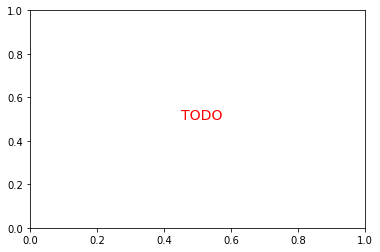
\includegraphics[width=0.5\textwidth]{Chapter3/Figures/todored}
	\caption{Data center topology used in simulations}
\end{figure}%
\\The first point is to generate a given amount of traffic. We want the hosts to fed the DCN with a given offered load $\rho$ defined as the average traffic offered to the switching fabric normalized to the bisection bandwidth. All hosts in the network have a single traffic source application and a single traffic sink application. Flows arrive at traffic sources according to a Poisson process with intensity $\lambda$ and are sent to a traffic sink belonging to another server chosen uniformly at random. Every new flow size is drawn from a given distribution. The flow size distributions that we considered are generally the ones already presented in section \ref{sec:workloads}. We did few experiments also with the uniform distribution at the very beginning to verify what happens when the flow size distribution has low variability. We never accounted for cases of heterogeneous workloads across the data center, thus all servers are always assumed to run the same workload. The bounded Pareto distribution wasn't available by default in the OMNeT++ library. However, it is easy to generate new samples of a random variable $X$ from any distribution through the CDF inversion technique. It is first extracted a uniform point $y \in [0,1]$. The uniform distribution is readily provided in the library of the simulator. Then, the following transformation involving the inverse of the cumulative function $F(x)$ is performed:
\[
x = F^{-1}(y)
\]
Essentially, the value $y$ is projected through $F(x)$ on the support of the distribution, giving the corresponding $y$-th quantile $x$, which is the new realization of the distribution of $X$ we needed. For the bounded Pareto with support in the interval $[u,t]$, whose $F(x)$ has been expressed in Eq.\ref{eq:bpcdf}, it holds:
\[
F^{-1}(y) = \sqrt{-\dfrac{(ut)^\alpha}{yt^\alpha - yu^\alpha - t^\alpha}}
\]
In order to implement the Poisson arrival process it has to be derived its intensity $\lambda$. Let $n_S$ be the number of spines, $n_T$ the number of ToRs and $n_H$ the number of hosts per rack. Denote with $C$ the link capacity connecting a rack with a spine. It has to be expressed the total traffic on the bisection bandwidth as a function of $\lambda$. First write the probability that a flow originated by a server in rack $T_i$ is destined to another server in a rack $T_j$ with $i \neq j$ (exit rack probability):
\[
P_{out} = \frac{(n_T-1)\times n_H}{n_T \times n_H - 1}
\]
Indeed there are $(n_T-1)\times n_H$ possible destinations among the total number of servers, excluded the source. If only cross-rack flows are simulated, obviously $P_{out}$=1.  Next, from the average flow size at application layer $\mathbb{E}[X_{(7)}]=\mathbb{E}[X]$ we need to obtain the average flow size at physical layer $\mathbb{E}[X_{(1)}]$. Define $\mathcal{H}(i)$ the procotol control information (PCI) added by the $i$-th OSI layer. The average flow size at physical layer is the average flow size at application layer with the addition of all headers in between. For a fixed packet size $pktsize$, that we always set to the Maximum Transmission Unit for the Ethernet ($pktsize$=1500B):
\[
\mathbb{E}[X_{(1)}] = \mathbb{E}[X_{(7)}] + \dfrac{\sum_{i=0}^{4}\mathcal{H}(i)}{pktsize}
\]
Since the all racks have the same workload, the total load $\rho$ on the fabric corresponds to the average traffic outgoing a single ToR.
\begin{equation}
	\label{eq:udp-load-generation}
	\rho = \dfrac{\lambda \; n_H \; \mathbb{E}[X_{(1)}]}{n_S \; C} P_{out}
\end{equation} 
Here it has been implicitly used the merging property of independent Poisson processes (PP), that states that merging multiple independent PP gives another PP with rate equal to the sum of individual rates. Inverting Eq.\eqref{eq:udp-load-generation} gives the final intensity $\lambda$ to be adopted by all hosts in the network: 
\begin{equation}
	\label{eq:lambda}
	\lambda = \frac{\rho \; n_S \; C}{n_H \; \mathbb{E}[X_{(1)}] \; P_{out}}
\end{equation}
We performed experiments both with TCP and UDP. The reasons will be explained in details when describing their setup. However, in writing the total traffic with Eq.\eqref{eq:udp-load-generation} it has to be accounted also for control packets of the TCP connections. We decided to disregard \texttt{SYN} and \texttt{FIN} packets, since they really have a negligible impact on the total traffic.  Instead, we considered \texttt{ACK} responses. All hosts of a rack send back an \texttt{ACK} in exchange of every received TCP packet, thus:
\begin{equation}
	\rho_{TCP} = \rho + \gamma \; \rho, \qquad \gamma = \dfrac{acksize}{pktsize}
\end{equation}
The same reasoning applies also if the delayed-ACK option of TCP is applied, but $\gamma$ must be rescaled accordingly.  \\
\subsubsection{Simulation length}
Once $\lambda$ is known, it is possible to derive the simulation time $t_M$ required to observe an average total number of flows $M$:
\[
t_s = \dfrac{1}{\lambda}\;\frac{M}{n_H \; n_T}
\]
The rough criterion we used for choosing $M$ is to tune its value depending on the tail of the flow size distribution and the "importance" of tail flows for the total load. In particular, we considered the mass-weighted function (\S \ref{sec:workloads} Fig. \ref{fig:mwf}) to understand how much traffic is carried by flow sizes corresponding to high percentiles. For instance, for both Pareto distributions we have seen that flow sizes corresponding to percentiles as high as 99-th still carry a lot of traffic (for data mining actually they carry almost all the traffic). Therefore, for these distributions unfortunately we should observe some amount of these tail flows to actually load the fabric at the average traffic $\rho$ that we impose a priori. In this respect, tail flows are important to be simulated. For example, let's suppose we decided --- by looking at the mass-weighted function --- that we want simulate at least 100 realizations of the largest 1\% flows. We need on average a total number of flow samples $M \ge 100 \mslash 0.01 = 10000$. Usually for the web search Pareto workload we used $M \sim O(10^{4})$. Note that another aspect to keep in mind is also the number of simulated flows per server, that is the ratio $M \mslash (n_H \; n_T)$. If the topology is very large, the total number of flows $M$ must be increased to avoid non-homogeneity across servers in the offered traffic. For this reasons, the data mining workload it is really not practical and often it has been ignored.
\subsection{Host configuration}
\label{sec:host-config}
All hosts in the network have one source client application, that generates flows according to the Poisson process, and one sink server application, that only receives flows in order to measure FCT, then discards their bytes. The host configuration changes a bit depending on whether we used TCP or UDP as transport. We run experiments with TCP and UDP, motivated by the noticeable difference among PS and FIFO discipline we observed in chapter \ref{ch:numerical-simulator} for SD-MLFQ. Indeed, the setting adopted for UDP at end hosts turned out to resemble the FIFO service discipline. 
\subsubsection{TCP}
\begin{figure}[!tb]
	\centering
	\captionsetup{width=.75\linewidth}
	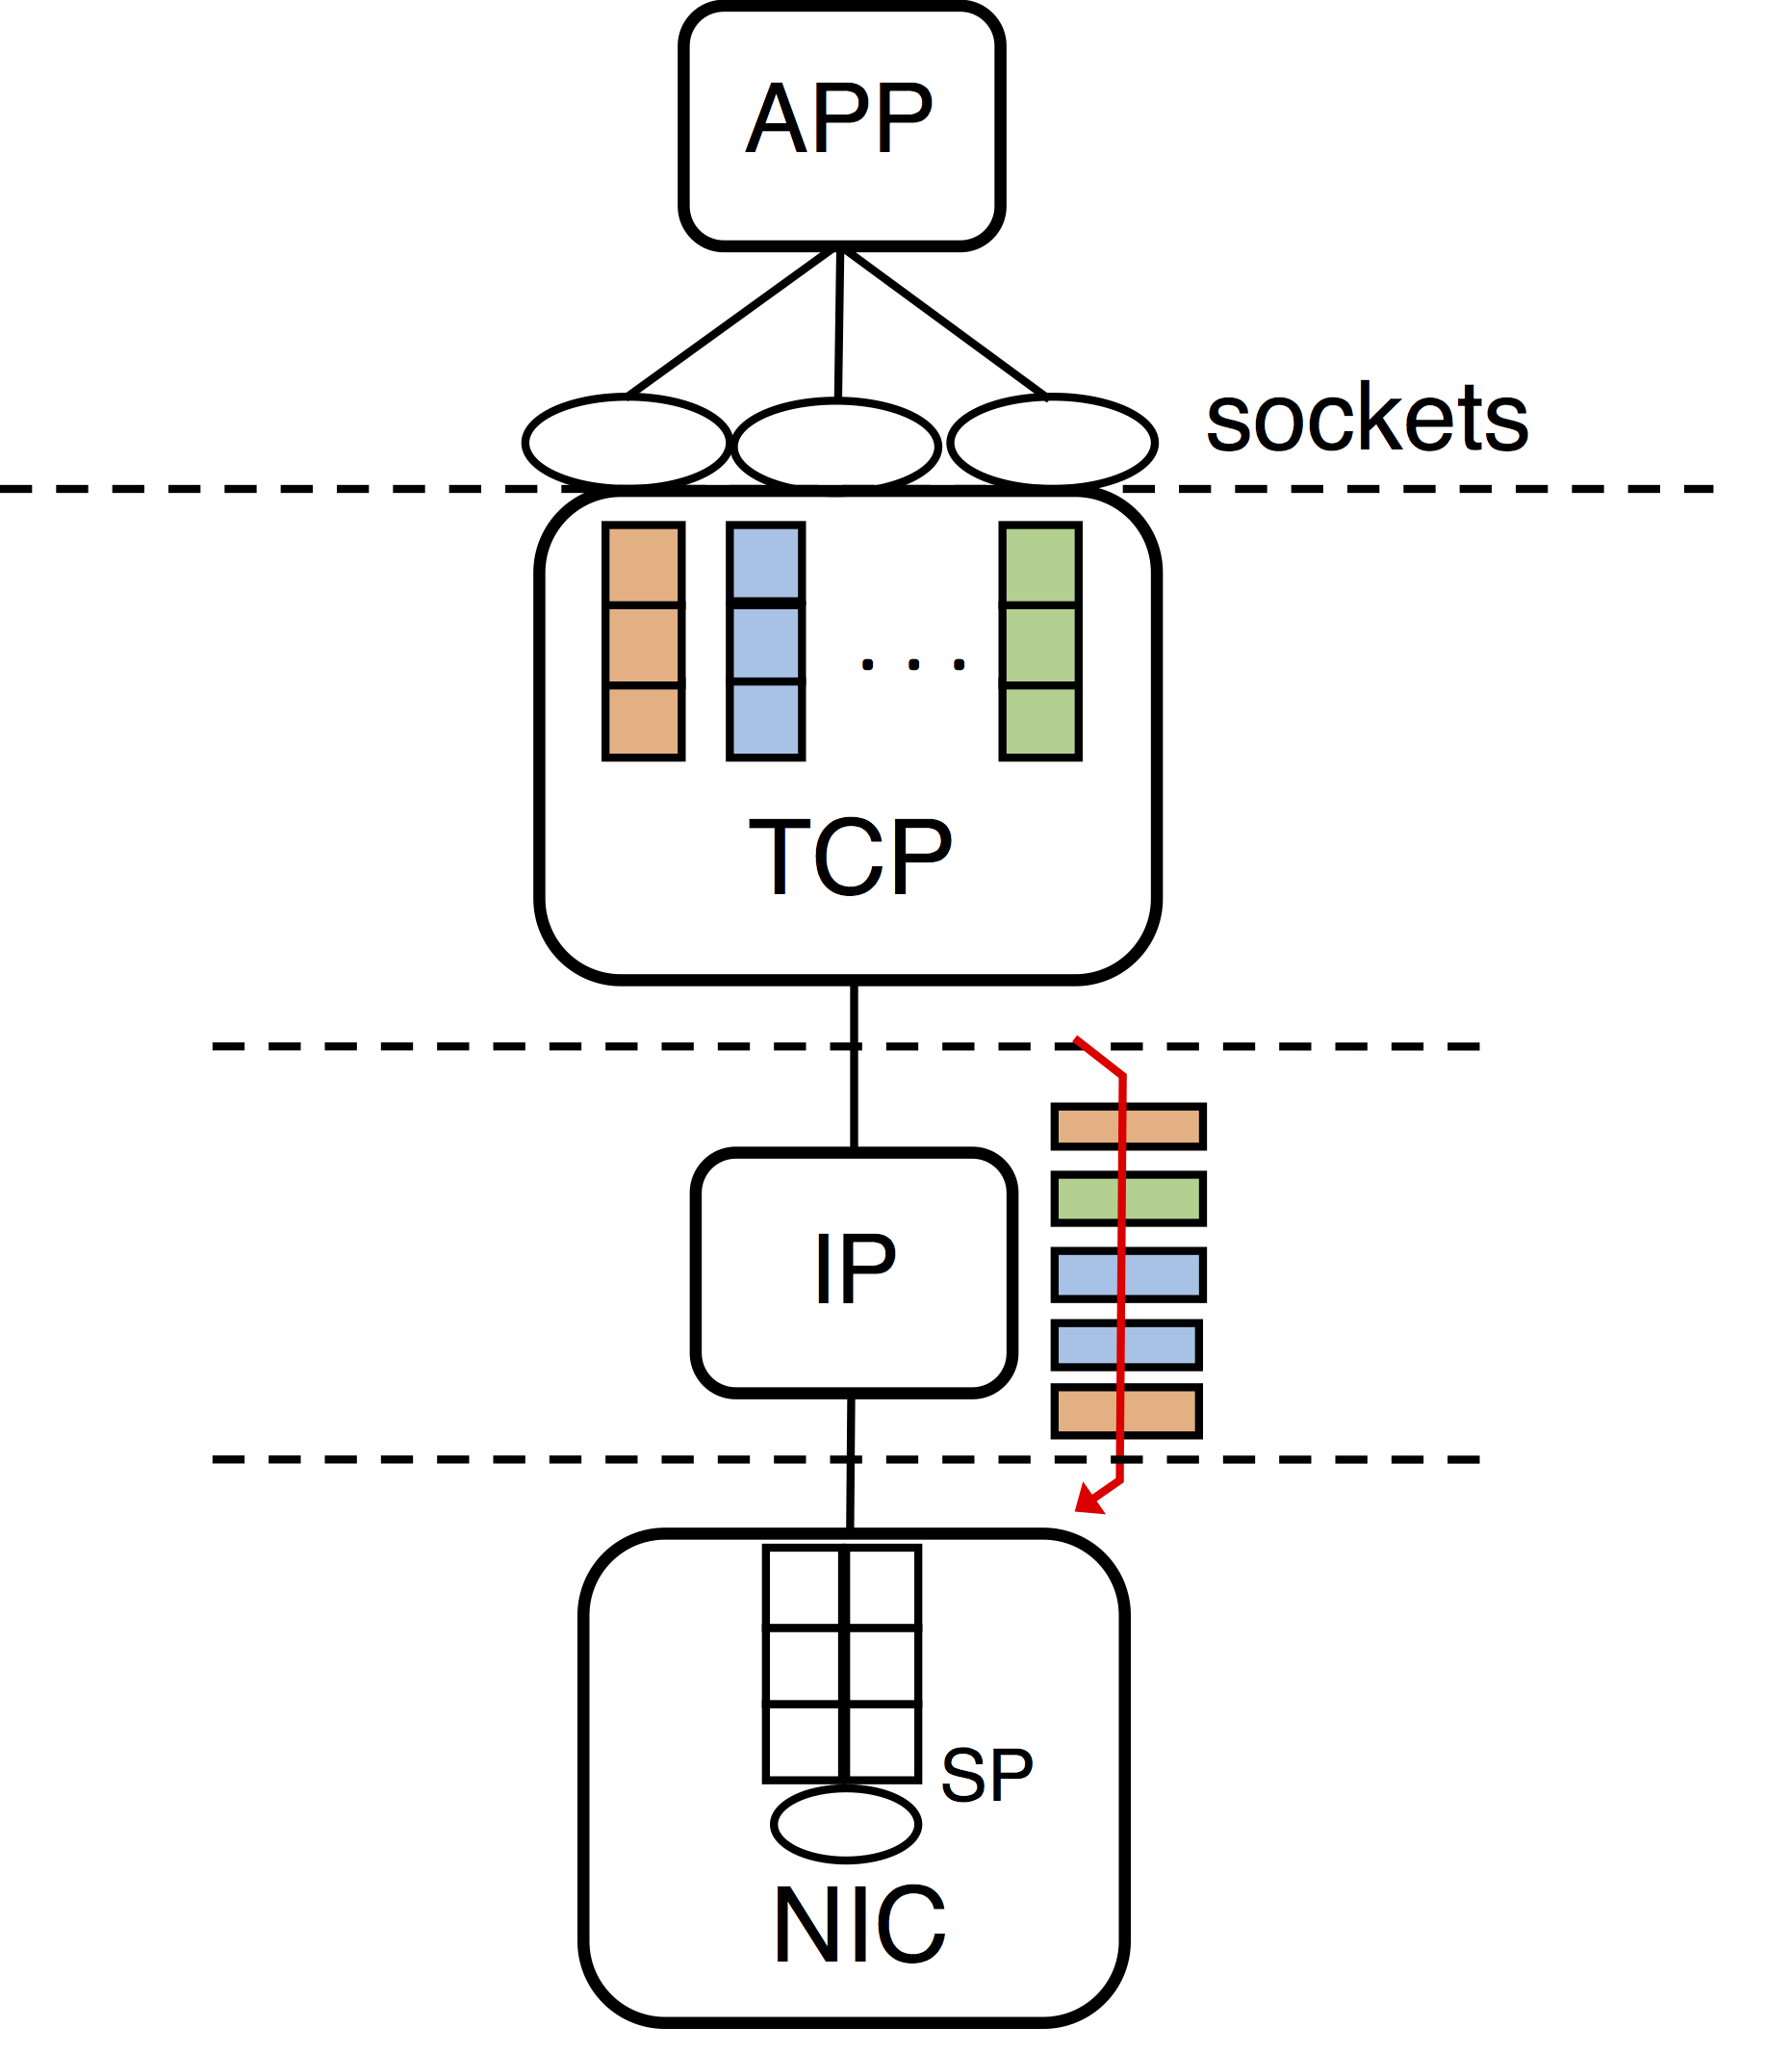
\includegraphics[width=0.4\linewidth]{Chapter4/Figures/tcp-config}
	\caption{Host architecture with TCP. Flows are interleaved thus emulating PS discipline.}
	\label{fig:tcp-config}
\end{figure}%
The architecture of the whole protocol stack at end hosts when adopting TCP is shown in Figure \ref{fig:tcp-config}. First start from the application layer. There is a unique application, following the generation process it setup a new TCP connection for each flow. Hence, already opened TCP sessions are not reused, but they are teared down when the flow completes. For every new connection, the application creates a socket, it batch sends the entire flow through the socket, offloading to TCP the segmentation in packets, then it immediately closes the socket. The application can close immediately the socket because it does not wait any data in response to its flow from the other peer of the TCP connection. There is not interaction, instead it only performs a one-way data transfer. For long flows this approach is not realistic. In a real TCP implementation the operating system would limit the maximum simultaneous bytes it can receive from the user application for preserving the memory allocation in kernel space. However, we can neglect these practical impairments to ease the implementation of the simulator. Opening and closing the socket in this way allows to avoid more complex management of simultaneous connection, like thread creation. Practically, our TCP application has been derived with some changes to the \texttt{TcpSessionApp} class of the standard INET library.\\
From the point of view of TCP, a separated transmission queue is allocated for each new socket. The simulator gave us the possibility to set the queue size limit to infinity. The scheduling among the queues is self-clocked by the TCP ACKs and transmission control mechanisms. A packet is popped from a queue only when the TCP window allow to do so. Simultaneous popping never occurs because ACKs belonging to distinct connections arrive back to back in the worst case. Therefore, packets of different flows are delivered to the IP layer with interleaving. When the socket transmission queue is completely drained, the TCP client immediately send a FIN packet for closing the connection, as the client application has already closed the socket. New connections always run the three-way-handshake during their setup and start with minimum window size. We do not set the initial window increase option of TCP. This is because the bandwidth-delay product of the network amounts to few packets. As a matter of fact, the distances between network elements in data centers are very short and propagation times on the network links are negligible for light speed. For example, on a link of 30m the bit propagation time is roughly 100ns. The transmission time of a TCP ACK packet on a 1Gbps link is 32ns. Thus, differently from large network on geographic scale, the Round Trip Time (RTT) is proportional to the packet transmission times. Since the topology is comprised by very few links, when multiplying the bandwidth and the RTT the result is near 5 packets.
We modified the defualt value of the TCP port range, in order to allow TCP to support the maximum number of simultaneous connection. With the default configuration, new connection could only use ports in the range 32768-61000. We extended the range to 1024-65535. Also, we removed the randomization of the initial sequence number, which is always started from zero. In this way, it is easy to discern the amount of service obtained by a flow and to tag its packets with the right priority. \\
Finally, we tackle at transport layer a possible shortcoming that has been also addressed in PIAS. Since we enforced strict priority queues also in the servers' NICs, that represent the first contention interface for the sender, large backlogs of packets may build up at end hosts. Indeed, the flows demoted to low priority stay active for long and many simultaneous flows share the server access link. They take time to converge to their fair share, meanwhile they increase their window to harvest additional bandwidth. The inet implementation of IP and MAC layer doesn't include back-pressure mechanisms to counteract the aggressiveness of TCP. Thus, either big delays or packet losses may be introduced yet before entering the network. A possible solution is to rate-limit to line rate the data flow between the application and the TCP. However, for the sake of simplicity we acted on the TCP Advertised Window (\texttt{AWND}) to upper bound the sender window to the bandwidth-delay product. Although the effect is practically the same, we are aware that in a real implementation the first solution is cleaner, because the bandwidth-delay product of the topology is in general unknown or not specified to the servers. 
\subsubsection{UDP}
\label{sec:udp-setup}
The scenario changes when adopting UDP as a transport protocol. Systems that aim to minimize the Flow Completion Time usually target transport protocols that ensure the delivery of the entire flow, thus neglecting UDP protocol. We tested the system also with UDP essentially for two reasons. First, it is easier to control its behavior, because it do not implement congestion control schemes, retransmissions, timeouts,..It is straightforward to check if the measured load on the topology corresponds to the offered load and verify the correctness of the traffic generation algorithm. Second, it may provide a rude approximation of the FIFO service at flow level, that gave the best results with spatial diversity (\S \ref{sec:dimensioning-spatial}). This is best understood considering Figure \ref{fig:udp-config}. It is well known that differently from TCP, UDP is connectionless. As a consequence, flows are packetized directly at application level and transfered to UDP already broken in datagrams. UDP does not have internal queues nor transmission control schemes, so it forwards all packets to IP, which in turn does the same with the MAC layer, that finally enqueues all packets in the line card buffers. In our simulator this happens in time zero, meaning that all these operations are code routines of the different layers that do not increase the simulation time. In other words, the new flow arrival event at application layer triggers all these network stack operations, which end only once all the packets of the flow are stored in the NIC's buffer. Since the simulator handles one event at a time, nothing else happens in the meantime. The relevant effect is that flows are served fully in FIFO order without interleaving at end hosts. In the network there is statistical multiplexing among different flows, even if the number of concurrent flows in the same interfaces is significantly reduced, due to the discipline enforced at the servers.\\
We use a trivial format for the application message, in order to make few information available on each UDP packet. In particular, we attach to application messages a sequence number and the flow length. Both the information are used for tagging packets with their priorities and to detect at the receiver when the flow is ended.
\begin{figure}[!tb]
	\centering
	\captionsetup{width=.75\linewidth}
	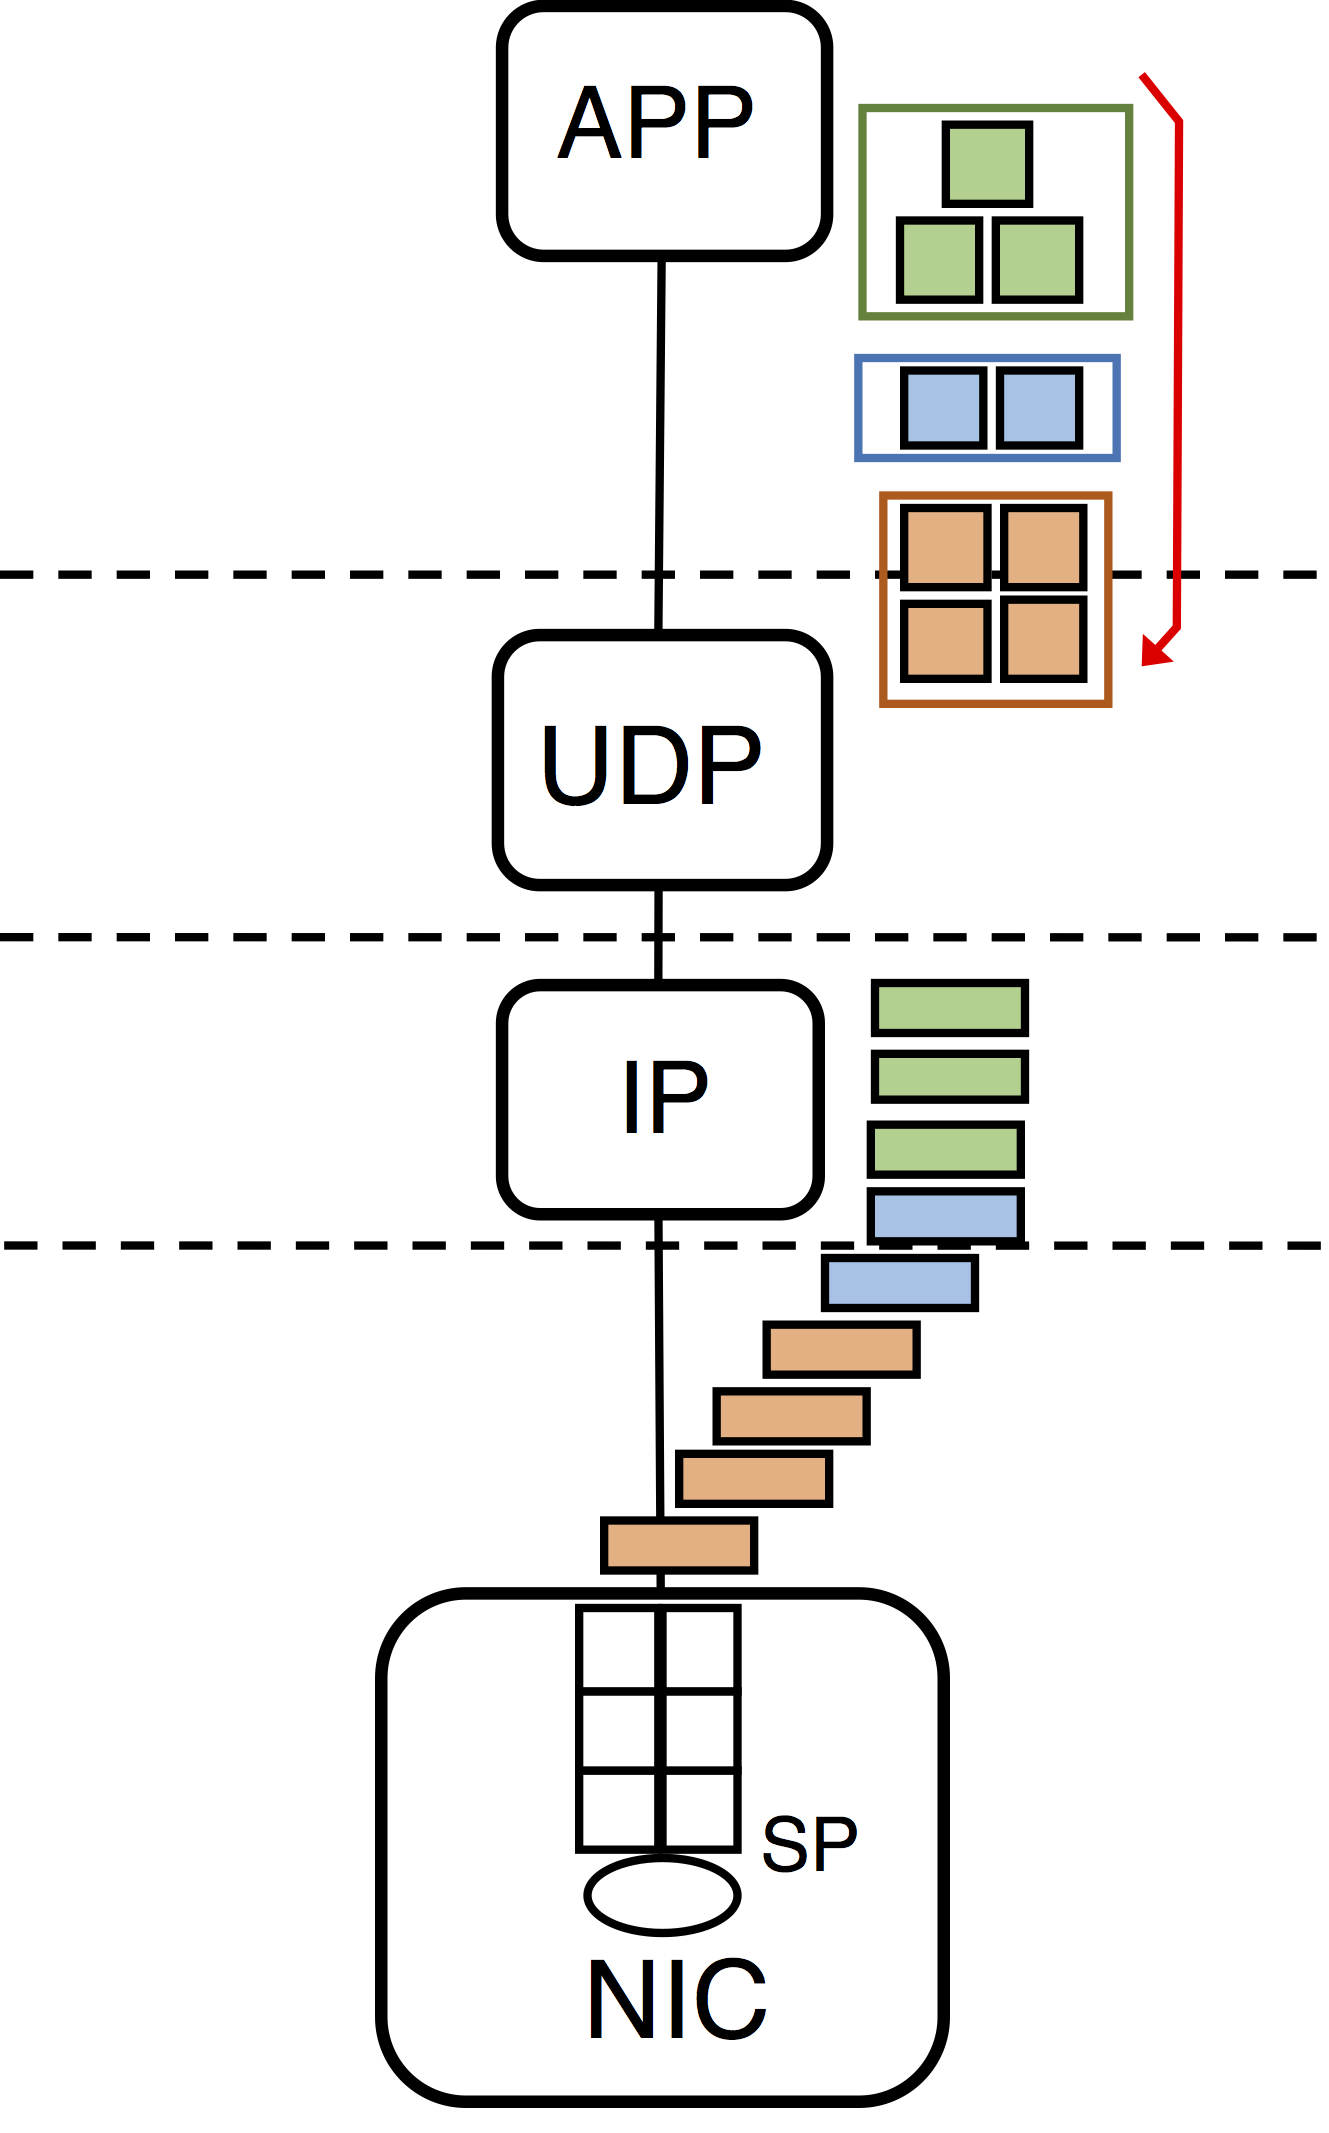
\includegraphics[width=0.3\linewidth]{Chapter4/Figures/udp-config}
	\caption{Host architecture with UDP. Flows are not interleaved thus emulating FIFO discipline.}
	\label{fig:udp-config}
\end{figure}%
\subsection{Network configuration}
% TODO modified djikstra
As discussed in chapter \ref{ch:sdframework}, a radical effect of SD-MLFQ is that the priority of a flow determines its routing over the topology. In a leaf-and-spine network, the ToR switches has to decide in which spine forward every packet, depending on some load balancing criterion. For SD-MLFQ, it is the flow priority, that has been assigned accounting for load balancing. Therefore spatial diversity has to be considered in routing algorithms. \\
We decided to handle the priority-dependent routing with a centralized controller module. End-hosts ask packet-by-packet to the central controller both the priority for their flows and the corresponding route. The controller knows the DC-wide flow size distribution and has computed all the demotion thresholds. Also, it keeps a centralized network view and it knows the priorities configured on every interface in the network. Thus, it can easily respond with a priority code and the route. The route depends on the load balance thresholds and it is provided as a vector of interface identifiers, whereas the priority code depends on the sub-thresholds. End hosts attach the interface IDs to their packets as a control information and tags the packets with the priority code. Finally, they send them through the network. The network devices use the interface identifiers for forwarding packets on the proper links and the priority to enqueue the packets on the proper priority queues. To sum up, it is applied a sort of source routing with the help of a central controller. \\
Both the route requests to the controller and the route information are handled offline, hence they don't contribute as overhead to network traffic. It means they are just data structures and function calls in the simulator. Instead, the priority code is carried in the DSCP field of the IEEE 802.1p \cite{ek1999ieee} standard for VLANs. This was the more immediate and flexible way to have a working prototype, without messing with solutions that make use of standard routing protocols to announce the priorities handled by the network nodes. The actual implementation of spatial diversity routing is out of the scope of this work. We think, however, that a centralized solution would be easy practicable also in modern SDN-based data center networks. \\
%Some changes were required to the inet modules in order to implement spatial diversity mechanism.
At this point, we built the entire topology using only standard inet modules for Ethernet switches with our modification for the forwarding-plane. We configured a single LAN for any topology size and we do not place any IP functionality inside the network. We do not need IP because the routing is handled by the controller. Also, we disabled the computation of the spanning tree and we instructed all servers with predefined entries in the ARP table before the beginning of the simulation. In this way we avoided all the possible problems that might arise from having a unique layer 2 network, such as spanning tree convergence or broadcast storms. Since we do not consider neither network nor server failures, the initial ARP mappings are valid for the entire simulation. We set priorities both at server and switch interfaces to implement the MLFQ scheduler. All priority queues are FIFO queues disciplined by a simple strict priority scheduler. Flow demotion is managed at the sources as explained above. Network switches are left with the only responsibility of choosing the priority queue by reading the DSCP code. \\
All links are Ethernet cables with a length of 30 meters, which seems reasonable in relation to the size of data center buildings. Buffer sizes are set to 1000 packets shared between priority queues of the same interface. Different ports have their own independent memories. We ignored switch architectures with port-shared memory pool, although they are common in data center networks \cite{dctcp, mqecn}.  In the experiments with UDP all queues have unlimited buffer space, in order not to loose packets and allow straightforward FCT measurements at the receiver. This is because packet losses would unnecessarily make controversial the meaning of FCT itself. Despite we are absolutely aware that the system with UDP has no practical value, nevertheless we recognize it has a theoretical utility.
\subsubsection{Priority assignment in down-send}
\label{sec:downsend-priority}
An aspect that we never addressed in the numerical simulator is how to assign priorities at the egress interfaces, that connect ToR switches to the servers. These ports are last traversed in the \emph{down-send} transmissions before leaving the switching fabric. During the up-send phase of the path from source to destination server we may exploit the spatial diversity to augment the priority classes proportionally to the number of spines. However, when traversing the egress interfaces all the priorities must be in some way mixed and multiplexed to the small number of queues available on a single port. This is illustrated in Fig. \ref{fig:downsend} for the case of rank=4 and two PQs per port, where 8 priorities have to be mapped on two queues. Our observation is that all egress interfaces receive the same DC-wide workload used for generating new flow sizes, because flows are uniformly sent to destination servers. Hence, we treat egress interfaces as in the system without spatial diversity, applying demotion at link level. In our experiments we mostly focused on 2 PQ, thus it was possible to compute rapidly the optimal PIAS threshold.
\begin{figure}
	\centering	
	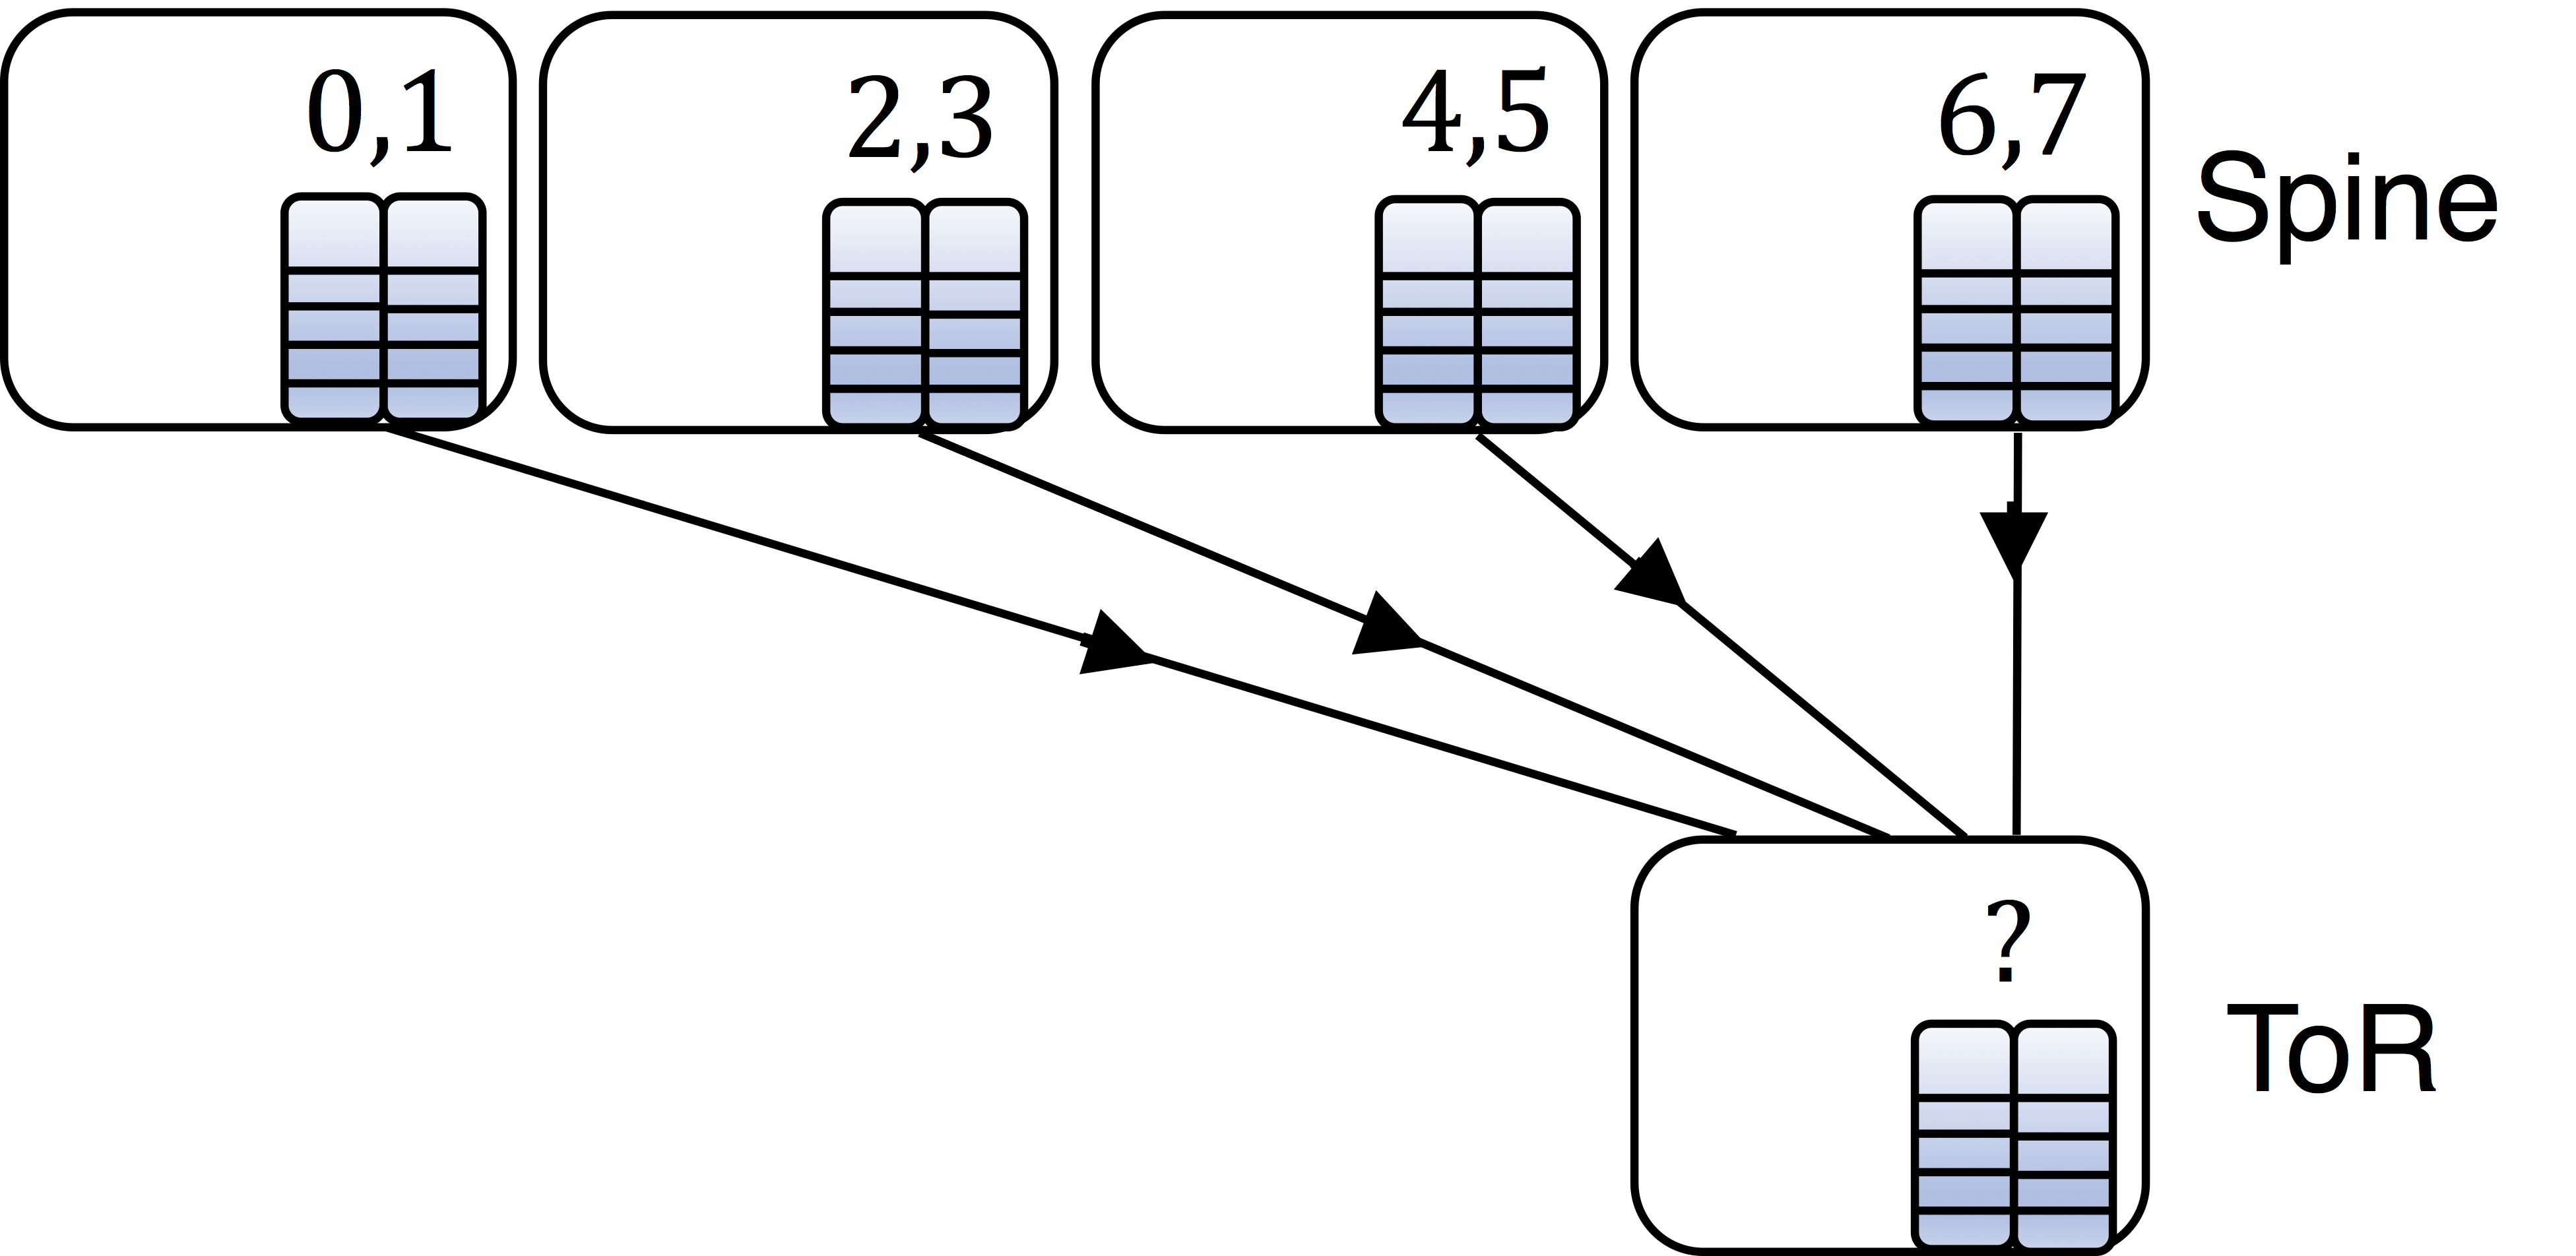
\includegraphics[width=0.5\textwidth]{Chapter4/Figures/downsend}
	\caption{Priority mixture in egress interfaces}
	\label{fig:downsend}
\end{figure}%
\subsection{Datacenter TCP (DCTCP)}
\label{sec:dctcp}
For the final versions of our experiments we employed state-of-the-art DCTCP \cite{dctcp}, among all possible versions of TCP.
Datacenter TCP (DCTCP) is a milestone for transport protocol design in data centers. It actually consists in minimal modifications to TCP New Reno. Its main insight is to leverage Explicit Congestion Notifications (ECN) from the network to properly modulate the window size of the TCP senders. The basic idea behind DCTCP is that queues in the network should be kept as empty as possible to avoid large backlogs that increase latency and do not leave enough headroom to absorb burst arrivals, occurring for example due to incast. Instead of pushing the window to grow until a packet drop is detected, the DCTCP transmitter slows down proactively depending on the level of congestion on the bottleneck link. Network queues mark packets with a congestion signal as soon they exceeds a given occupancy $K$. Then, TCP receivers convey back the congestion signals to TCP transmitters, setting the ECN-Echo bit to 1 in their ACKs. Finally, the TCP sender mantains an estimate $\alpha$ of the fraction of marked packet on an interval of roughly one RTT and modulates the window as:
\[ \text{cwnd} = \text{cwnd} \times (1-\alpha/2)\]
This way, upon mild congestion the window size is gently reduced --- note that only in case $\alpha$=1 it is cut in half as in standard TCP --- still ensuring high throughput, but mitigating its aggressiveness.\\It has been proven that DCTCP effectively succeed in lowering the amplitude of queue oscillations to $O(\sqrt{\text{BDP}})$, instead of $O(\text{BDP})$ of TCP, being BDP the bandwidth-delay product, while not losing throughput for a proper setting of the marking threshold $K$. More importantly, the queue length with DCTCP is proven to be predictable with an analytical expression. In the worst case of $N$ synchronized flows, the queue length is stable around $K+N$. \\
Note that the only requirement from the network is to configure switches with an AQM scheme to mark packets. In practice this can be achieved configuring the RED algorithm, already available in most devices, so that it marks based on the instantaneous queue length and with a unique high and low threshold equal to $K$. 
\subsubsection{DCTCP testbed}
We implemented the above changes to TCP in INET and the ECN markers to plug into the switch interfaces. We deployed the same testbed used in the original article of DCTCP \cite{dctcp}, in order to verify the correctness of the implementation. The testbed topology is shown in \ref{fig:dctcp-testbed-topology}. A group of $N$ server (on the left) start simultaneously long-lived TCP connections towards the same destination server (on the right). We used $N=2$ and $N=20$ and flow sizes fixed to 100MB. All links are configured at 1Gbps speed and the DCTCP parameters set according to the guidelines of the reference paper. In particular, the threshold $K$ is set to 20 packets. \texttt{AWND} is set to its maximum value, so that the transmission control is not restricted. Buffer sizes are set to 500 packets.\\ 
\begin{figure}
	\centering
	\begin{subfigure}{.35\textwidth}
		\centering
		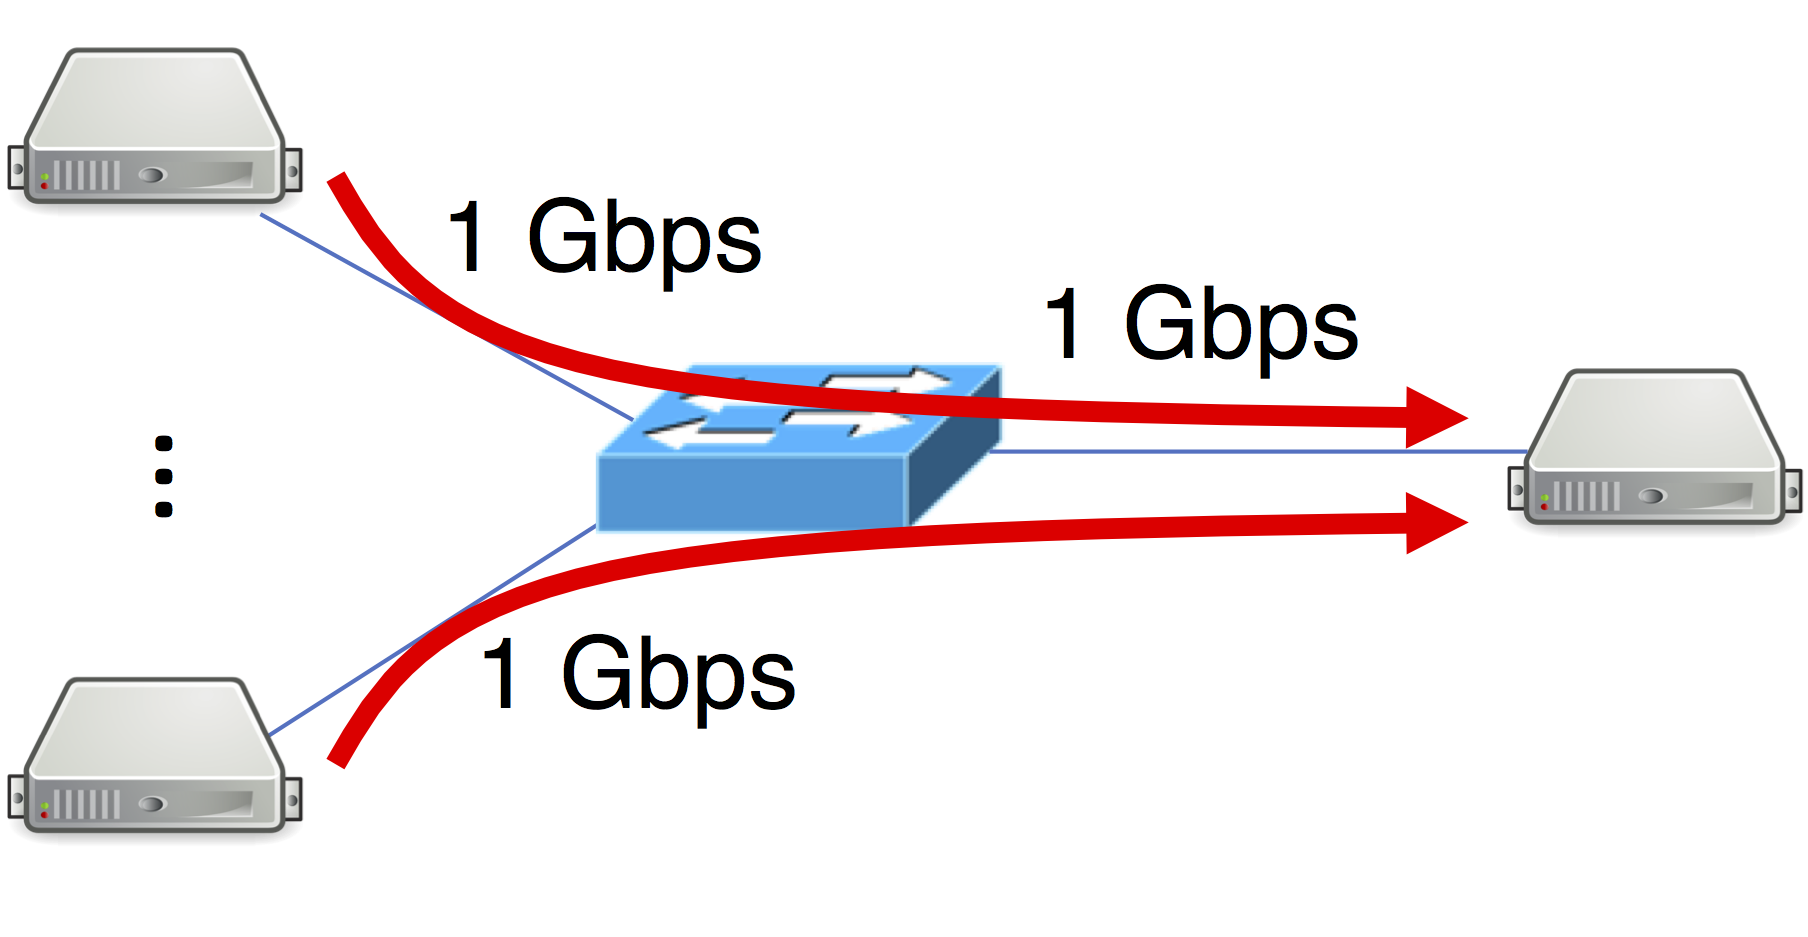
\includegraphics[width=0.99\textwidth]{Chapter4/Figures/dctcp-testbed}
		\caption{Testbed topology}
		\label{fig:dctcp-testbed-topology}		
	\end{subfigure}%
	\hfill
	\begin{subfigure}{.65\textwidth}
		\centering
		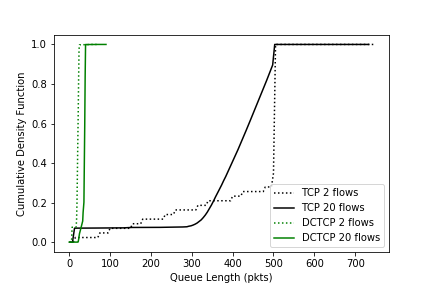
\includegraphics[width=0.9\textwidth]{Chapter4/Figures/dctcp-qlen}
		\caption{CDF of queue length, sampled every 10 packets}
		\label{fig:dctcp-testbed-res}		
	\end{subfigure}%
	\caption{DCTCP implementation testbed}
	\label{fig:dctcp-testbed}
\end{figure}%
We compare the CDF of the queue length when using TCP New Reno and DropTail queues in the bottleneck interface, with the case of DCTCP and ECN-enabled buffers (Fig. \ref{fig:dctcp-testbed-res}).  
It is clearly appreciable the effectiveness of DCTCP, which enforces the queue length to be stable around the predicted value. Conversely, with TCP DropTails the queue variance enlarges significantly, indicating the presence of large oscillations typical of sawtooth pattern induced by TCP AIMD congestion control scheme.
\subsubsection{Integrating ECN with SD-MLFQ}
We set ECN markers only in the network switches with recommended \cite{dctcp} threshold value. Conversely. servers have been equipped with simple DropTail queues and do not adopt AQM schemes. We dealt with few caveats in order to seamlessly integrate ECN rate control with the SD-MLFQ simulator. \\
\textbf{Per-port ECN marking}. First we had to choose how to apply ECN marking to the multi queue scenario. There are fundamentally two choices that trade latency, throughput and fairness. One possibility is to configure the recommended marking threshold independently on each of the $N$ priority queues available. This solution is known as per-queue ECN. It guarantees full link utilization in each priority queue, but the total queue length could potentially grow $N$ times larger and introduce high delays especially to low priority packets. Another option, referred to as per-port ECN, adopts a single marking threshold shared among different priority queues. While ensuring low latency, per-port ECN doesn't provide isolation among queues. Prior work \cite{mqecn} proposed dynamic threshold adjustment to provide best trade-off. We chose to simply use per-port ECN following the same approach as in PIAS. Per-port ECN could help in mitigating the long flow starvation problem. Starvation on low priority queues is undesirable with TCP, since it triggers retransmission timeouts of the connections even if the packets are not lost. Ultimately, it may lead to abrupt connection termination. With per-port ECN and its shared threshold, large buffer pressure on low priority queues helps in slowing down high priority traffic. \\
\textbf{Marking \texttt{SYN/ACK} with CE codepoint.}
According to standardization \cite{ipecn}, ECN capable devices can mark with the congestion signal (\texttt{IP\_CE} - Congestion Experienced codepoint in the IP ToS field) only those packets with the  ECN Capable Transport codepoint set (\texttt{IP\_ECT} codepoint). However, the standard ECN extension to TCP specifies that control packets (\texttt{SYN, ACK, FIN},.) must been transmitted as Non ECN-Capable (\texttt{IP\_NOT\_ECT} codepoint). Thus, if they enter a switch interface when its occupancy exceeds the marking threshold, they are dropped rather than being marked. We noticed in our first simulations with DCTCP an anomalous number of retransmission timeouts (RTOs). We better investigated the number of bytes transmitted at the time when TCP connections experienced RTOs: practically all timeout events occurred at connection setup. These timeouts are particularly long because the TCP hasn't yet estimated the network RTT and applies a conservative value, whose default is absolutely oversized for the RTT of a DCN. Consequently many connections never started but remained in timeout state along the entire simulation. To rapidly overcome the issue we implemented the modification to TCP that allows ECN-Capable control packets \cite{synecn}.
\section{Result analysis}
This last section will be a walkthrough of the results obtained with the data center network simulator, including a few initial experiments that do not concern directly spatial diversity, but rather emphasize the importance of the assumptions we made about the flow size distribution. \\
We will mainly focus on small topologies, since the numerical model highlighted the restraints in applying spatial diversity with high number of spines. In particular, for the final evaluation of spatial diversity we will consider 2x2, 3x3, and 5x5 topologies, with the notation $n_T \times n_S$. The same phenomena observed in the numerical queuing model started to appear also in the data center when considering the 5x5 topology, thus we do not considered larger topologies. Notice that due to the modularity of the data center network, spatial diversity could be also applied to large scale topologies by repeating the $n_T \times n_S$ configuration in parallel many times. This concept has already been introduced in the definition of SD-rank (\S \ref{sec:dimensioning-spatial}). 
\subsubsection{Adversarial traffic distribution for MLFQ}
In the first stages of this work during the deployment of the simulator, we enforced the hosts to generate traffic according to a simple uniform distribution. Our scope was just to verify the correct implementation of the load generation algorithm and of the strict priority scheme with demotion.  However, we faced several issues especially in controlling the load in the network. We measured mismatched between the load offered by application layer and the actual link utilization. We realized that TCP is particularly sensitive to the adoption of MLFQ and network performances may be severely deteriorated without a careful parameter settings if the flow size distribution does not exhibit high variability. Some traffic distributions are particularly adversarial to the MLFQ scheduler, mainly because they conflict with the strict priority scheme. It is known that strict priority could introduce starvation and packet drops to low priority flows. In the MLFQ such a starvation does not appear since the beginning of the flows but suddenly after their demotion, because initially all flows are handled at high priority. The TCP congestion control suffers this situation: the RTT changes abruptly, many timeouts expire (Fig.\ref{fig:num-rto}) and unnecessary retransmissions are injected in the network. Retransmissions are counted as transmitted bytes by the priority tagger, thus they further increase low priority traffic and ultimately exacerbate the problem. Also, the transmission window of starved flows is throttled due to persistent congestion, so these flows have low throughput even when the scheduler grant them the link bandwidth and higher priority queues are empty. 
\begin{figure}
	\centering
	\begin{subfigure}{.5\textwidth}
		\centering
		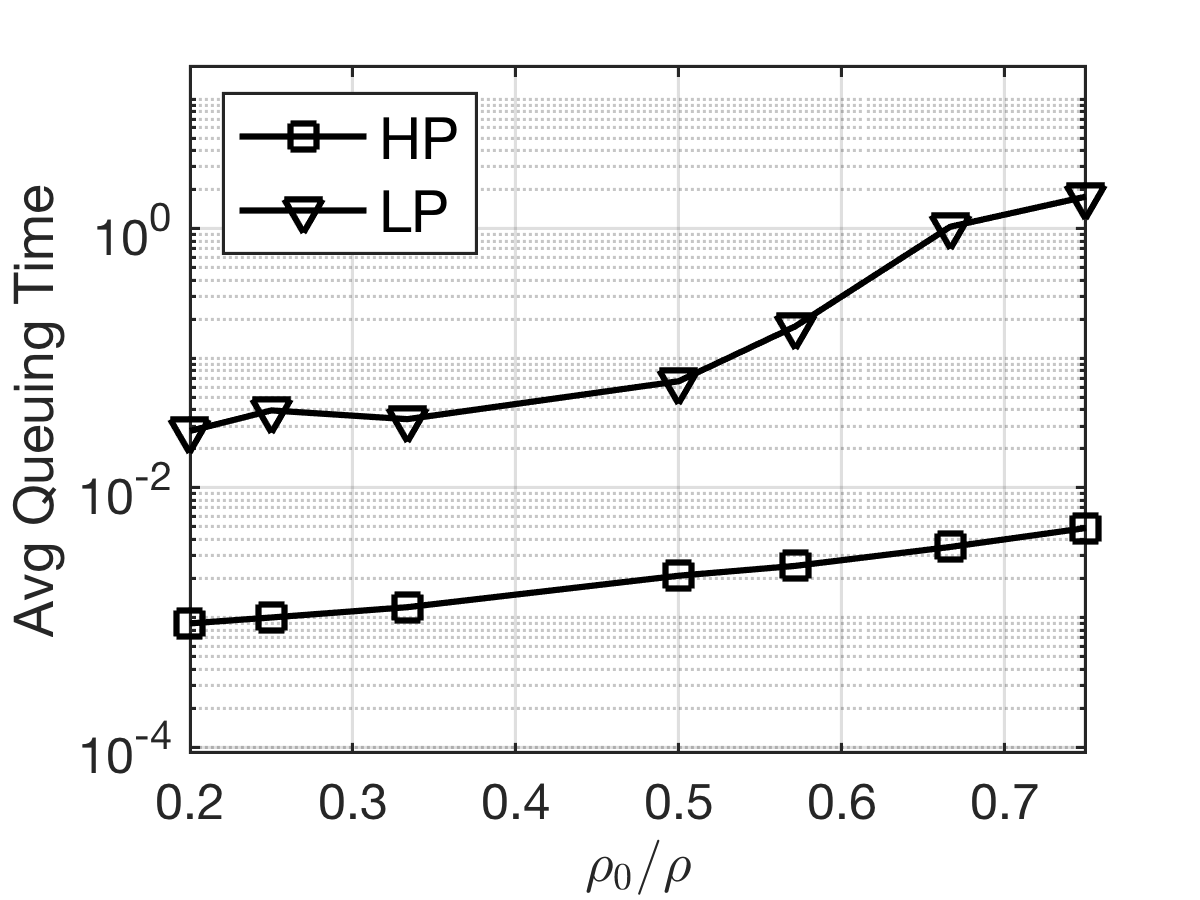
\includegraphics[width=0.8\textwidth]{Chapter4/Figures/qt_vs_thresh}
		\caption{Queuing time ($\rho=0.9$)}
		\label{fig:qt-vs-threshold}
	\end{subfigure}%
	\hfill
	\begin{subfigure}{.5\textwidth}
		\centering
		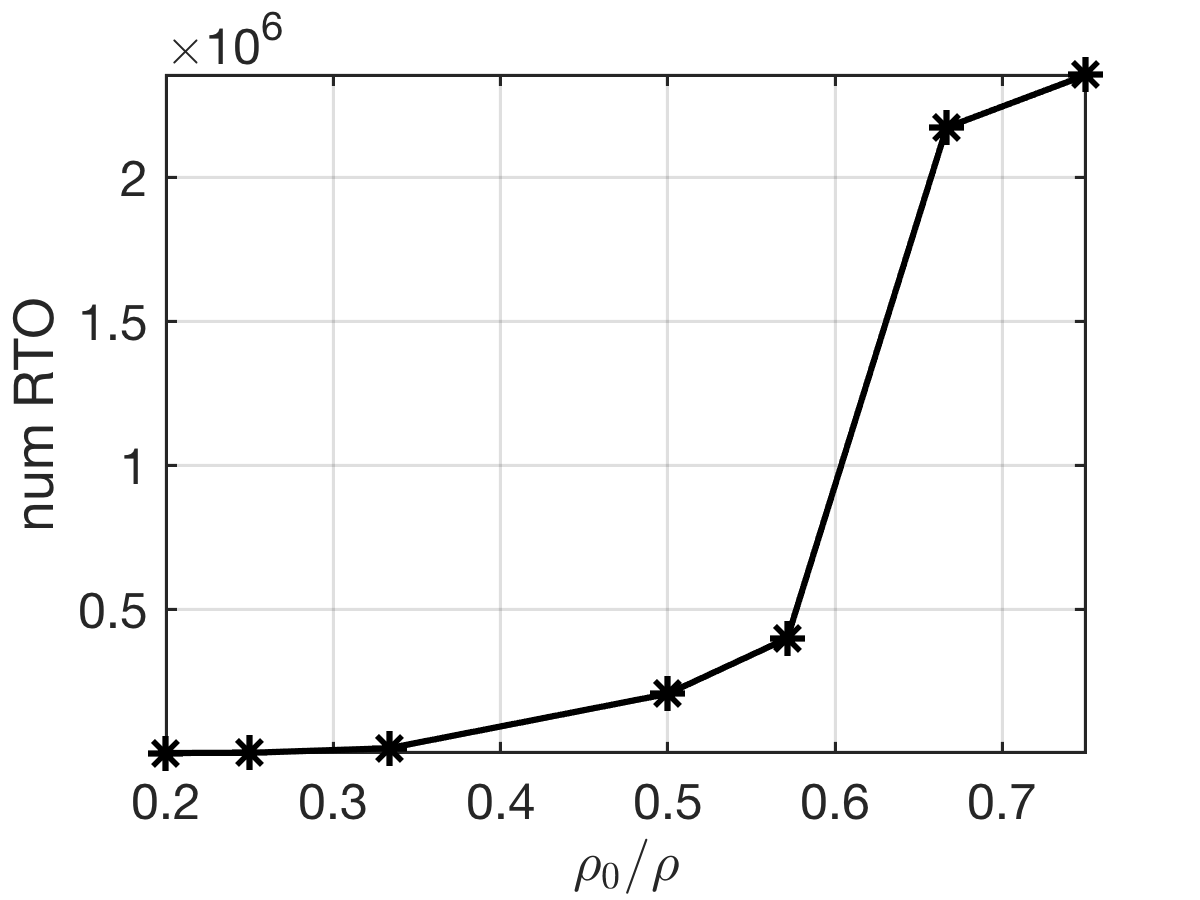
\includegraphics[width=0.8\textwidth]{Chapter4/Figures/rto_vs_thresh}
		\caption{TCP timeouts}
		\label{fig:num-rto}
	\end{subfigure}%
	\caption{Impact of traffic apportioning among PQs on TCP}
	\label{fig:uniform-traffic-sp-tcp}
\end{figure}%
However, the main issue with a uniform flow size distribution is that many of low priority flows are continuously generated with the same probability of other flows. Thus a relevant portion of flows ends up in the low priority queues, whose sizes grow, boosting the starvation loop. On the contrary, for heavy-tailed distributions long flows are a small percentage, therefore the queue size remains under control. \\
For all these reasons, under adversarial traffic distribution the MLFQ system is very susceptible to the threshold setting and the behavior of TCP becomes difficult to control.
% TODO
% defintion of nomenclature for interfaces and devices
% link speeds and clear topology definition
% better description of analytical model PIAS
% acknowledgments prof
% abstract, intro, conclusion
% plot of pias vs las vs srpt vs...
% djikstra modified (would be nice)
% change DSCP not true actual field is VLAN PCP!!!
% change section titles according to Paolo's insights
% HPC ack
% UDP with 1 priority queue
% Spatial diversity problem of priority "inversion"
% SD with bigger topology 5x5 what happens ..?
To better investigate the starvation problem of strict priority queuing with TCP and uniform traffic distribution, when working close to saturation ($\rho \sim 0.9$), we tested a simple system with $N$=2 priority queues and we vary the values of a single threshold $\alpha$. 
In particular, we fixed the ratio $\rho_{0} / \rho$, where $\rho_0$ is the load on high priority queue and $\rho$ is the total load on the interface $\rho_{0} + \rho_{1}$. We chose the value of $\alpha$ by solving the load balance equation \eqref{eq:main-K-PQ} for MLFQ. For uniform distribution with support in $[a,b]$:
\begin{equation*}
\alpha = b - \sqrt{(b^2 - a^2)(1-\dfrac{\rho_{0}}{  \rho})}
\end{equation*}
The testbed topology in this case had $n_T=2$ and $n_S=1$, $n_H=10$. As usual, no oversubscription is applied. We measured the average queuing time at the egress interfaces. %TODO table with interface names and deifnition of access links / aggregation links
When $\rho_{0} / \rho$ gets sufficiently high, the lower priority queue (LP) is served less frequently.  Starvation starts to appear for $\rho_0 / \rho > 0.5$ (Fig. \ref{fig:qt-vs-threshold}), where the average queuing time rises exponentially. The opposite doesn't happen: when the majority of the load $\rho$ feeds the lower priority queue, HP does not starve because strict priority scheduling always prioritize traffic on HP, even if LP is more utilized. 
\subsubsection{Effects of priority queue granularity without spatial diversity}
Upon the above understanding, we neglected any traffic distribution different from the workloads commonly used in literature. We carried out experiments with the web search workload, in order to verify the gains achieved when increasing the priority queue granularity in the system without spatial diversity. Moreover, it was of our interest to directly analyze the shape of the nFCT curve in respect to all the flow sizes (Fig. \ref{fig:esn_varying_N}), instead of the global average only. This breakdown is not always provided (at least not for PIAS and pFabric). However, we think that showing only the global average or just three separated averages for mice, medium and elephant flows is not exhaustive and in general depends on the way these categories are derived, which is arbitrary. We define mice flows the ones with size (0B,100KB], medium flows with size (100KB, 10MB] and elephant (10MB, $\infty$]. This classification is common in literature \cite{pias, nos2, one-more-queue}.\\
\begin{figure}
	\centering
	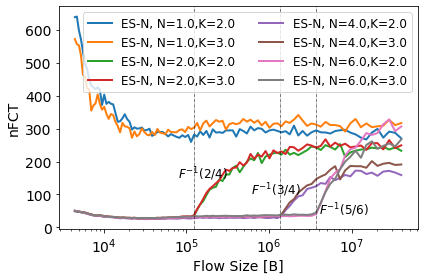
\includegraphics[width=0.6\textwidth]{Chapter4/Figures/esn}
	\caption{MLFQ with ES-N thresholds for different $N$ and $\rho$=0.9}
	\label{fig:esn_varying_N}
\end{figure}%
We obtained Figure \ref{fig:esn_varying_N} by averaging FCT with a custom binning of flow sizes, in order to get a similar number of samples on each bin. The technique we used for choosing bin edges was to split the cumulative function of the flow sizes, $F(x)$, into uniform intervals and evaluate the inverse of $F(x)$ at the interval bounds. The clear trend evinced is coherent with the outcomes of reference works. The priority granularity affects most of all medium sized flows, which do not get mixed immediately with long flows in the lowest priority queues, as it happens for $N$=2. Mice flows, instead, have a huge gain when passing from 1 to 2 priority queues, then their response time is essentially untouched. Vertical axes show the ES-N thresholds corresponding to given percentiles and remark the effect of strict priority as they are in correspondence of a sharp transition of the response time. Last, we observe some slowdown for mice flows when there isn't prioritization. This is most likely due to the higher impact of TCP control packets on these flows, which are comprised by no more than 10 packets.
\subsubsection{Optimized load balancing}
Next, we started to really evaluate spatial diversity in the data center network. In Sec.  \ref{sec:final-comparison} the best results for spatial diversity were obtained with the setting of a single priority queue per interface. In that case, by optimizing the load balancing and physically splitting shorter from longer flows, spatial diversity achieved better FCT than a system with random load balancing among spines. Moreover, the absence of strict priority scheduling relieved of flow synchronization and elephant demotion impairments. We expected to observe similar benefits also in the real data center network, however we discovered some shortcomings that make our approach ineffective in most cases. \\
\begin{figure}
	\centering
	\begin{subfigure}{.25\textwidth}
		\centering
		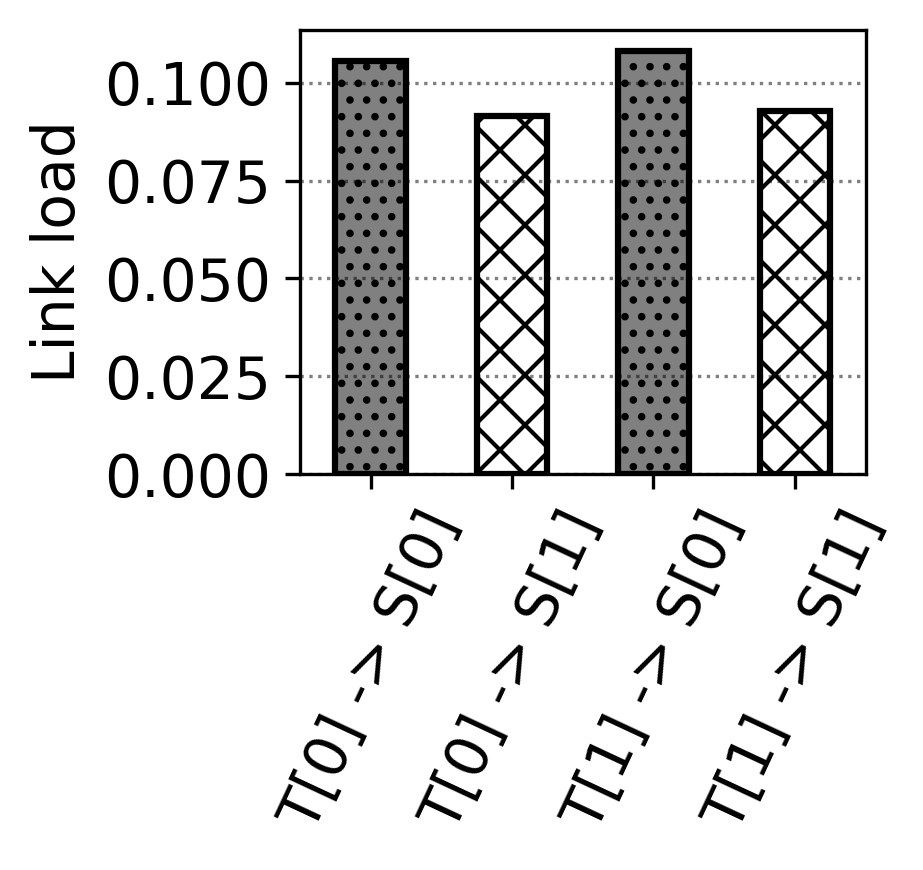
\includegraphics[width=0.99\textwidth]{Chapter4/Figures/opt_lb_lambda_01}
		\caption{Load 0.1}
	\end{subfigure}%
	\hfill
	\begin{subfigure}{.25\textwidth}
	\centering
	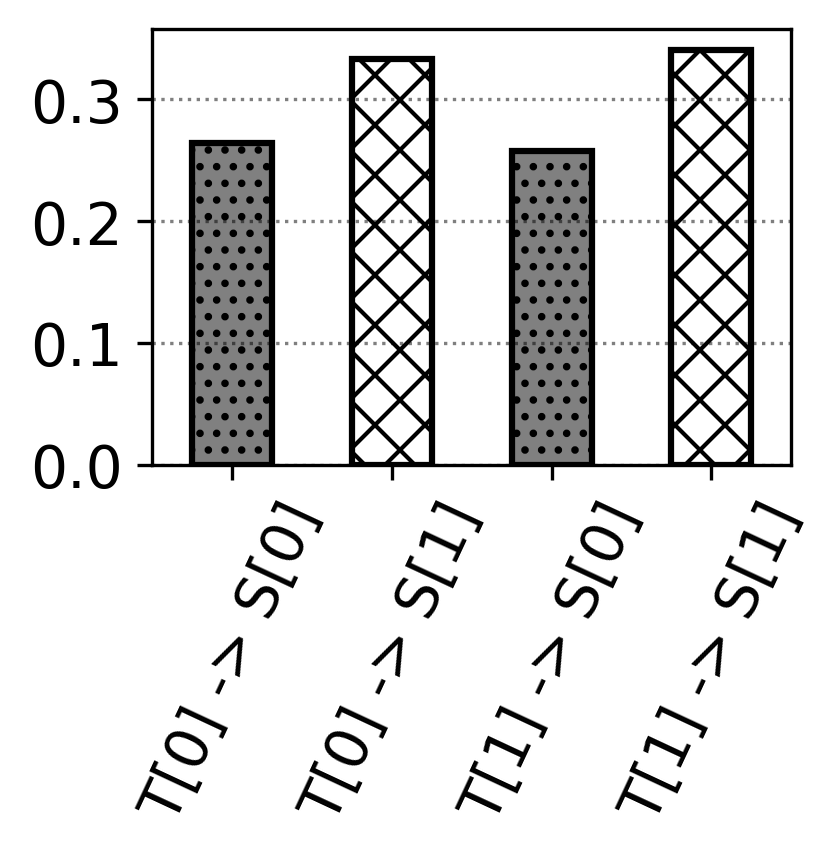
\includegraphics[width=0.92\textwidth]{Chapter4/Figures/opt_lb_lambda_03}
	\caption{Load 0.3}
	\end{subfigure}%
	\hfill
	\begin{subfigure}{.25\textwidth}
	\centering
	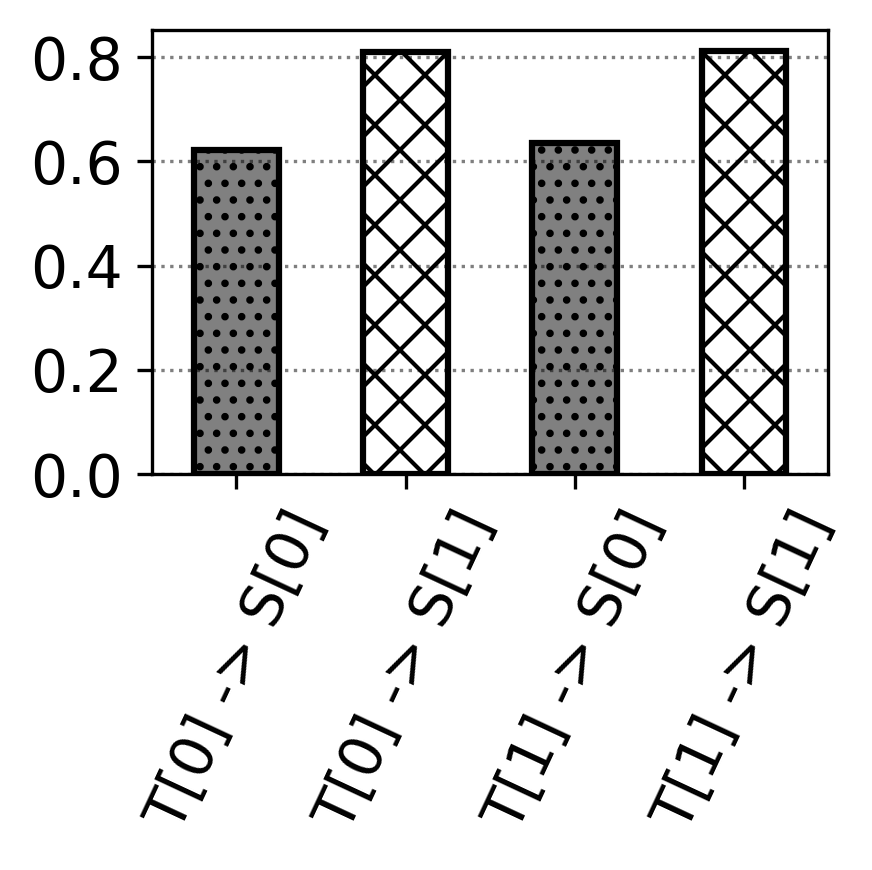
\includegraphics[width=0.92\textwidth]{Chapter4/Figures/opt_lb_lambda_07}
	\caption{Load 0.7}
	\end{subfigure}%
	\hfill
	\begin{subfigure}{.25\textwidth}
	\centering
	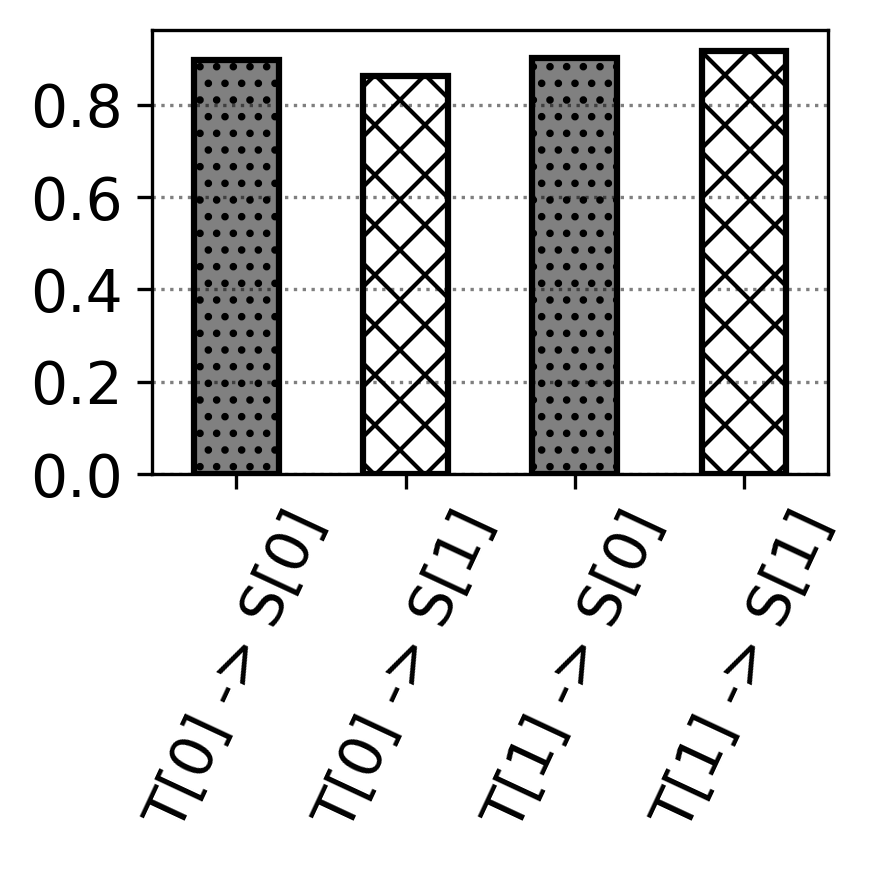
\includegraphics[width=0.92\textwidth]{Chapter4/Figures/opt_lb_lambda_09}
	\caption{Load 0.9}
	\end{subfigure}%
	\caption{Optimal vs ECMP load balancing with TCP}
	\label{fig:load-distrib-spines}
\end{figure}%
We compared two systems, without priorities and with different load balance strategies. The first system employs flow-level load balancing with standard ECMP, whereas the second system moves flows across spine after they have transmitted an amount of bytes corresponding to the optimal demotion thresholds computed in \ref{sec:decoupling}. We verify that the traffic is actually splitted among available spines according to the theoretical optimal split that we impose. Figure \ref{fig:load-distrib-spines} illustrates the traffic measured on the bisection links exiting from the ToRs, for different offered loads. For the sake of simplicity the figure refers only to the 2x2 topology, despite the following results will also include the 3x3 topology, where some trends are more evident. Nicely, the traffic follows exactly the same pattern we derived analytically, showed in Figure \ref{fig:perspineload-ws} of previous chapter. At low load the high priority spine $s_0$ is the one which receives most of the traffic, then starting from 30\% load the opposite happens, finally at very high load the traffic is load balanced almost uniformly. However, differently from the results obtained in the numerical model, the optimized load balance does not provide significant gains in terms of completion time, not only, it looses poorly at high load.
\begin{figure}[!tb]
	\centering
	\begin{subfigure}{.33\textwidth}
		\centering
		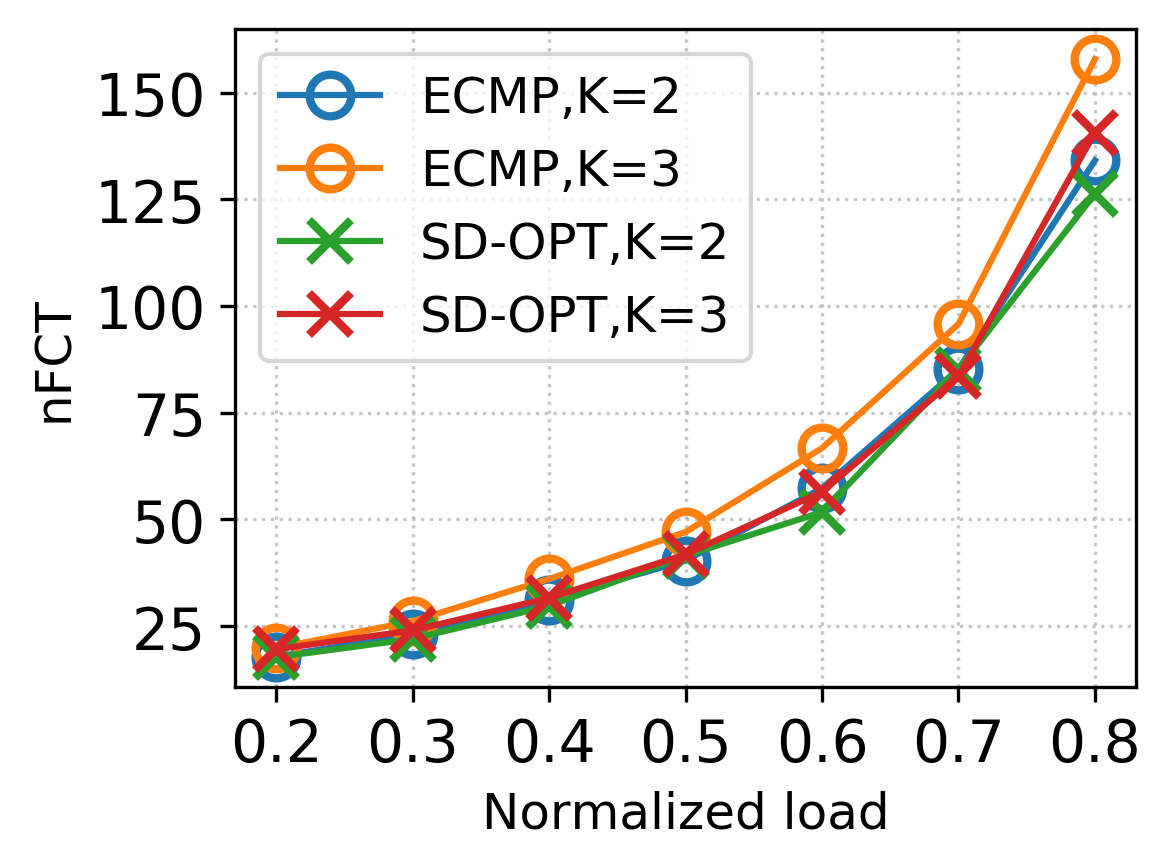
\includegraphics[width=0.99\textwidth]{Chapter4/Figures/optimal_lb_thresh_K_2_3}
		\vspace{1.4pt}
		\caption{Average FCT}
		\label{fig:opt-vs-ecmp-fct}
	\end{subfigure}%
	\hfill
	\begin{subfigure}{.33\textwidth}
		\centering
		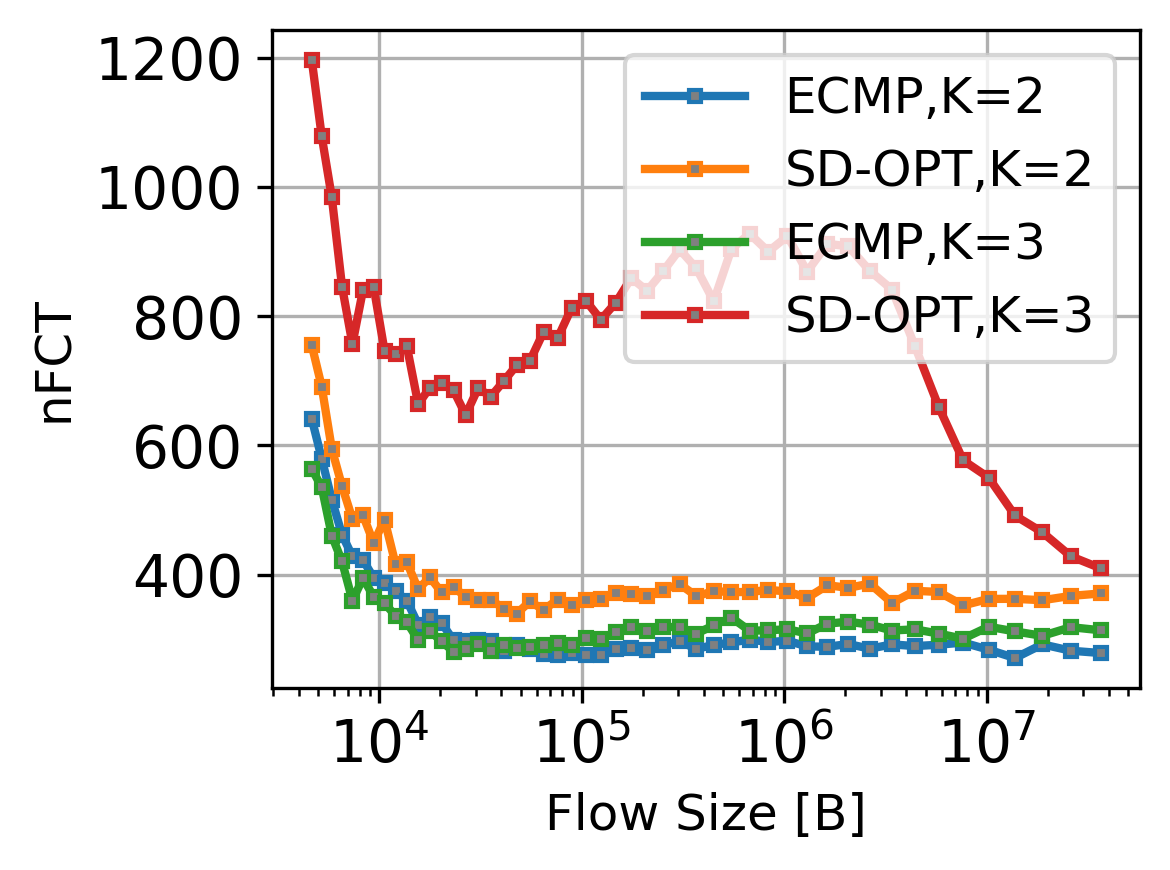
\includegraphics[width=0.99\textwidth]{Chapter4/Figures/optimal_lb_thresh_K_2_3_detailed}
		\captionsetup{justification=centering, width=0.7\linewidth}
		\caption{FCT detailed ($\rho$=0.9)}
		\label{fig:opt-vs-ecmp-fct-detailed}
	\end{subfigure}%
	\hfill
	\begin{subfigure}{.33\textwidth}
		\centering
		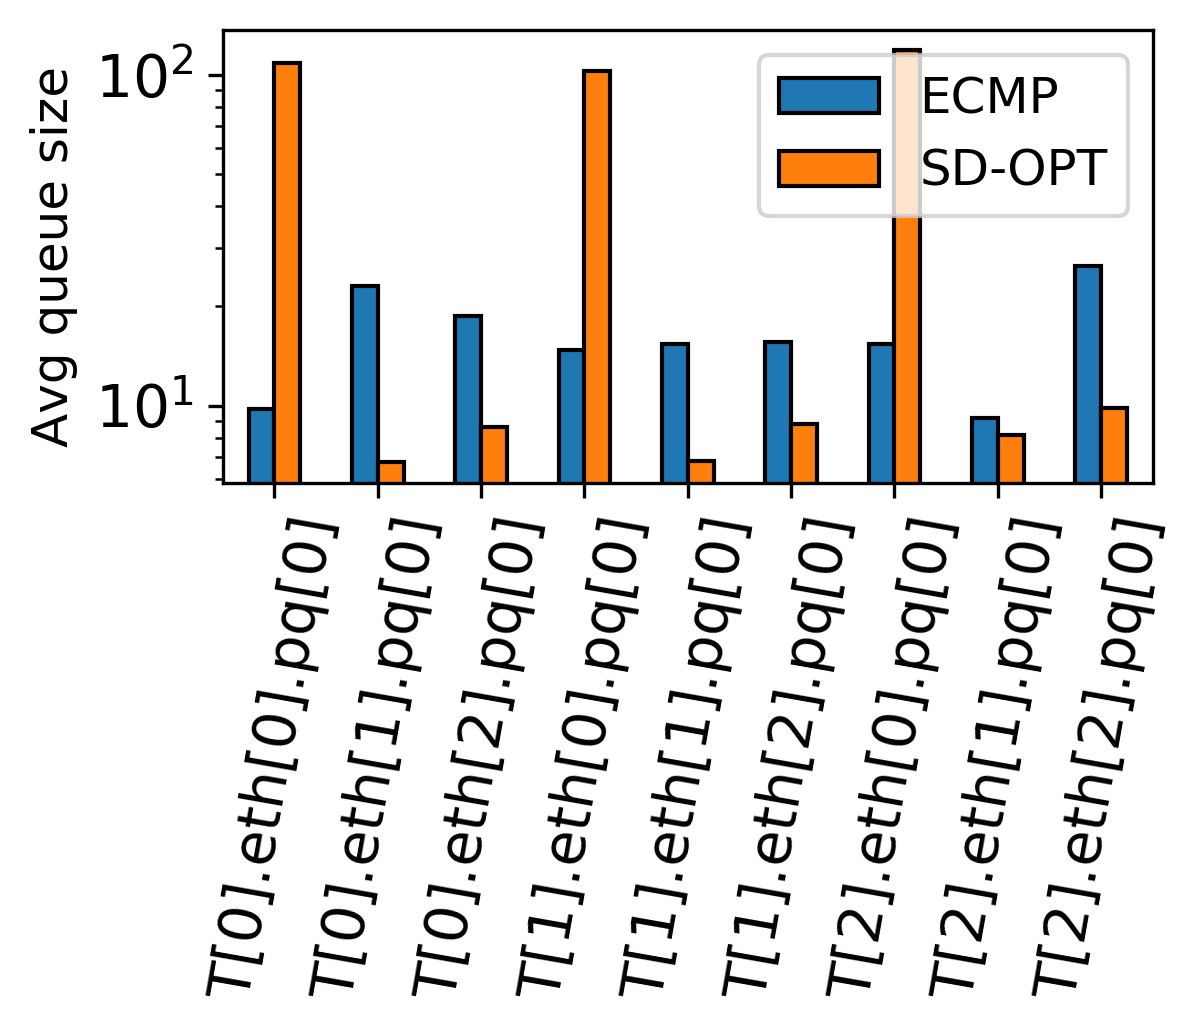
\includegraphics[width=0.99\textwidth]{Chapter4/Figures/queue_peaks_N_1}
		\caption{Queue peaks ($\rho$=0.9)}
		\label{fig:opt-vs-ecmp-queue-peaks}		
	\end{subfigure}%
	\caption{Optimal vs ECMP load balancing with TCP}
	\label{fig:opt-vs-ecmp-lb}
\end{figure}%
The exhaustive comparison is shown in Fig.\ref{fig:opt-vs-ecmp-fct}. For all loads except $\rho$=0.9 the performances are almost equivalent, with little advantages in using the optimal thresholds. On the contrary, at 90\% load the optimized load balancing is strongly penalized, especially with 3 spines (Fig.\ref{fig:opt-vs-ecmp-fct-detailed}). This was quite surprising since it differs a lot from what occurred with numerical simulations. We explained such a behavior by delving into the average queue lengths in the network interfaces. At 90\% load, there are visible peaks in all the interfaces towards high priority spine $s_0$ in the optimized load balance scenario. These queues on average are occupied almost ten times more than in the ECMP case. An equivalent plot --- not shown --- has been obtained for the down-send interface from spine switches to ToR switches for the 3x3 topology. For the 2x2, instead, such queues are empty because there at most only one rack transmitting to any other rack and its transmissions are shaped at the up-send interface connecting the rack to the spine. This is also the reason why in Fig. \ref{fig:opt-vs-ecmp-fct-detailed} SD-OPT with $K$=2 is a factor 2 better in respect of $K$=3. Unfortunately, we realized that this increased queue occupancy on the low priority spine is a side-effect inherent to spatial diversity, where all flows start their service in $s_0$. We gave the following explanation. Even if at load 0.9 all spines receive almost the same traffic, in terms of connections $s_0$ handle a notably higher flow arrival rate in respect to all other spines and several simultaneous TCP connections. Indeed, the majority of flows are short for our heavy-tailed workload, thus only a smaller and smaller number of flows end in subsequent spines. Although we didn't enabled the increased initial window option of TCP and all connections start at the minimum window, they all together combine on these queues, which grow large. Notice that the application of rate control policies such as DCTCP is almost useless, as it acts on the window of a single connection but do not reduce the connection arrival intensity. Also remember that DCTCP guarantees a queue occupancy around the sum of the marking threshold and the number of synchronized connections. Moreover, many flows of our workloads last only few packets, not enough to react to ECN marking. On the contrary, ECMP distributing new flows evenly among spines, does not suffer the same issue. Coherently with this analysis, on the links towards other spines $s_1$ and $s_2$, few parallel connections share the capacity and the average queue size is even smaller for SD-OPT than ECMP load balancing. \\
We did not observe the same issue in the numerical simulator because it was designed as a fluid approximation. The capacity of the spine processor was subdivided among all flows, which immediately started receiving service upon arrival, as opposed to the DCN where the packet granularity enforces some waiting time. Moreover, in the fluid simulator the jobs were entirely available to the queue since their arrival, not regulated by transmission control schemes like TCP which sends packets clocked by the receiver's signaling.\\
\begin{figure}[!tb]
	\centering
	\begin{subfigure}{.33\textwidth}
		\centering
		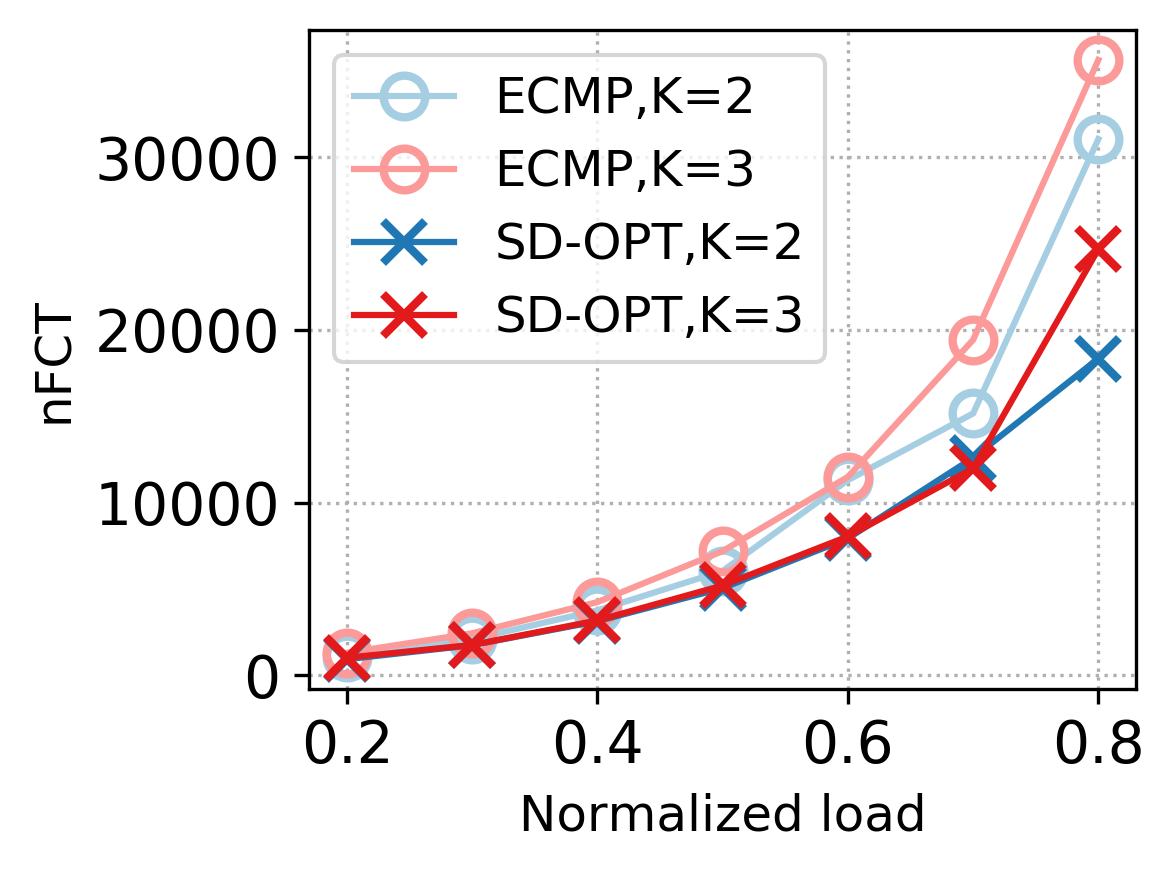
\includegraphics[width=0.99\textwidth]{Chapter4/Figures/optimal_lb_thresh_K_2_3_udp}
		\vspace{1.4pt}
		\caption{Average FCT}
		\label{fig:opt-vs-ecmp-fct-udp}
	\end{subfigure}%
	\hfill
	\begin{subfigure}{.33\textwidth}
		\centering
		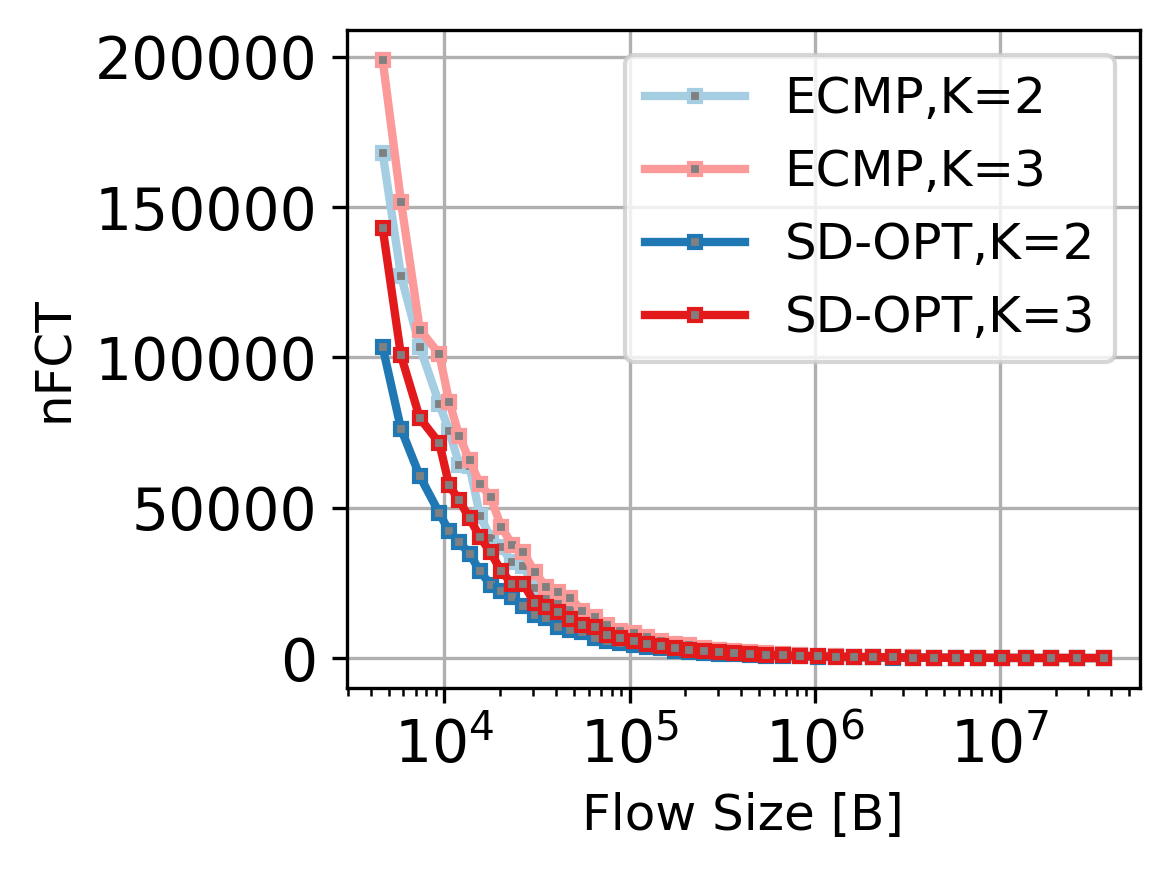
\includegraphics[width=0.99\textwidth]{Chapter4/Figures/optimal_lb_thresh_K_2_3_detailed_udp}
		\captionsetup{justification=centering, width=0.7\linewidth}
		\caption{FCT detailed ($\rho$=0.9)}
		\label{fig:opt-vs-ecmp-fct-detailed-udp}
	\end{subfigure}%
	\hfill
	\begin{subfigure}{.33\textwidth}
		\centering
		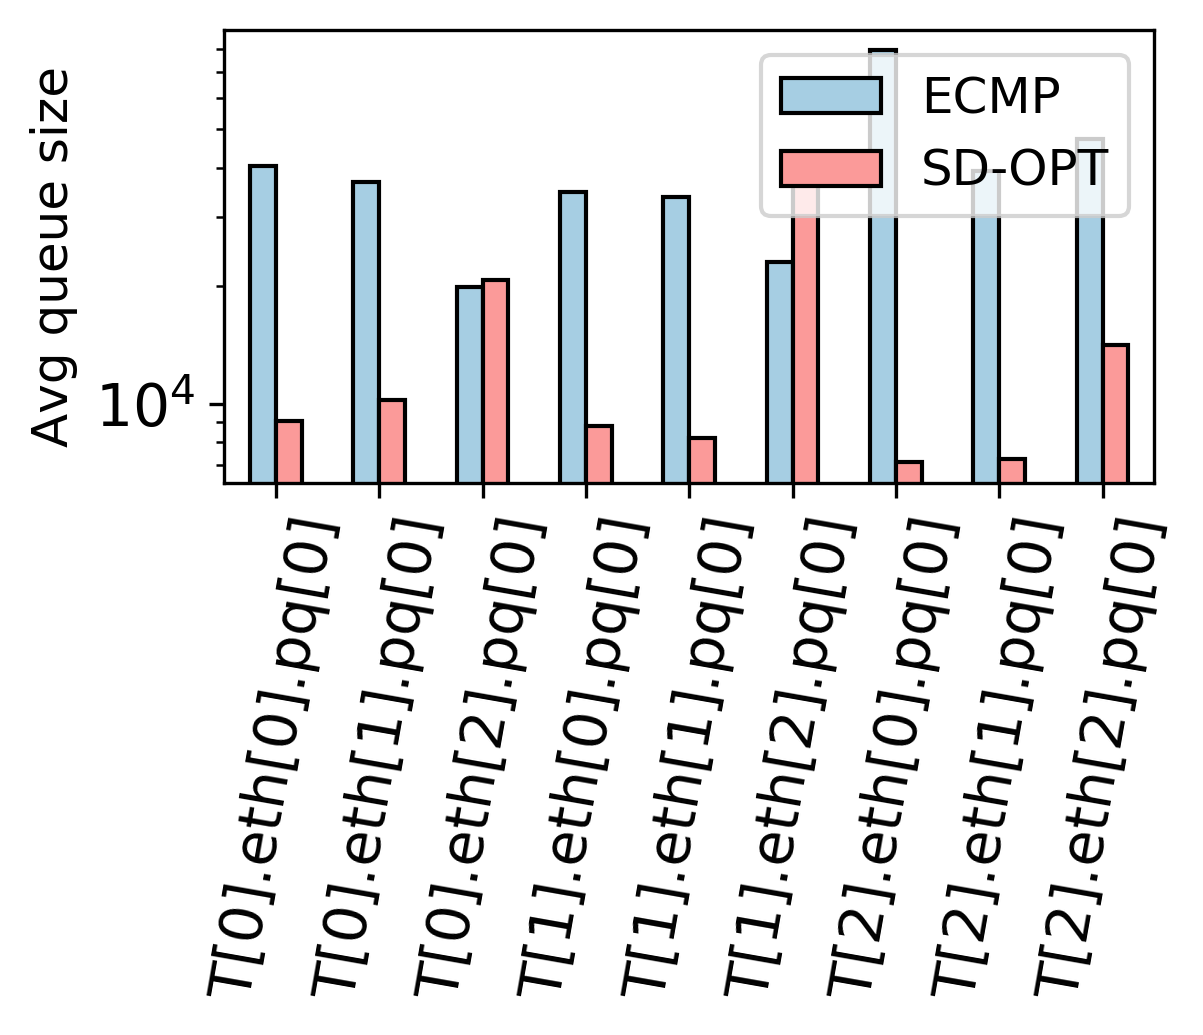
\includegraphics[width=0.99\textwidth]{Chapter4/Figures/queue_peaks_N_1_udp}
		\caption{Queue peaks ($\rho$=0.9)}
		\label{fig:opt-vs-ecmp-queue-peaks-udp}		
	\end{subfigure}%
	\caption{Optimal vs ECMP load balancing with UDP}
	\label{fig:opt-vs-ecmp-lb-udp}
\end{figure}%
We repeated the same experiment with UDP, configured as in Sec. \ref{sec:udp-setup}. In this case, flows are served in FIFO order without preemption at the servers line-cards. Consequently, short flows undergo a large slowdown because are queued back long flows (Fig.\ref{fig:opt-vs-ecmp-fct-detailed-udp}). Here the inter-spine demotion gives less pronounced benefits than in the FIFO flow simulator. Indeed, our UDP configuration mimic FIFO flow scheduling only at access line-cards, whereas inside the network packets of different flows are statistically multiplexed, thus flows are served in PS. However, the more interesting comparison is provided in Figure \ref{fig:opt-vs-ecmp-queue-peaks-udp}. The disproportionate peaks appearing with SD-OPT in TCP are not present with UDP. This is because the FIFO policy at the transmitter reduces consistently the flow arrival rate and the number of simultaneous connections on the low priority spine. New flows waits in the servers' line-cards before entering the network, until flows ahead complete. 
\subsubsection{Performances of SD-MLFQ with priorities}
Finally, we proceed in the evaluation of the MLFQ extension with the addition of spatial diversity, in presence of multiple priority queues per interface. We adopt always 2 PQ and we compare topologies with $K$=2,3,5. Load balance thresholds are optimized according to \ref{sec:optimal-lb-problem}, whereas sub-thresholds are chosen with the greedy \textit{Load-Split-N} algorithm that splits half of the traffic on high priority queue and half of the traffic on low priority queue (\S.\ref{sec:subthresh-with-sd}). First, we validate what discovered in the numerical model, that is augmenting the spatial diversity rank leads to worse completion times. This is shown in Figure \ref{fig:sdmlfq_varying_K} and in details in Figure \ref{fig:sd-final-detailed}. Indeed, with high SD-rank the shortcomings of spatial diversity --- such as flow synchronization and variability reduction for low priority spines (\S \ref{sec:sd-impairments})--- are more penalizing. \\
\begin{figure}[!tb]
	\centering
	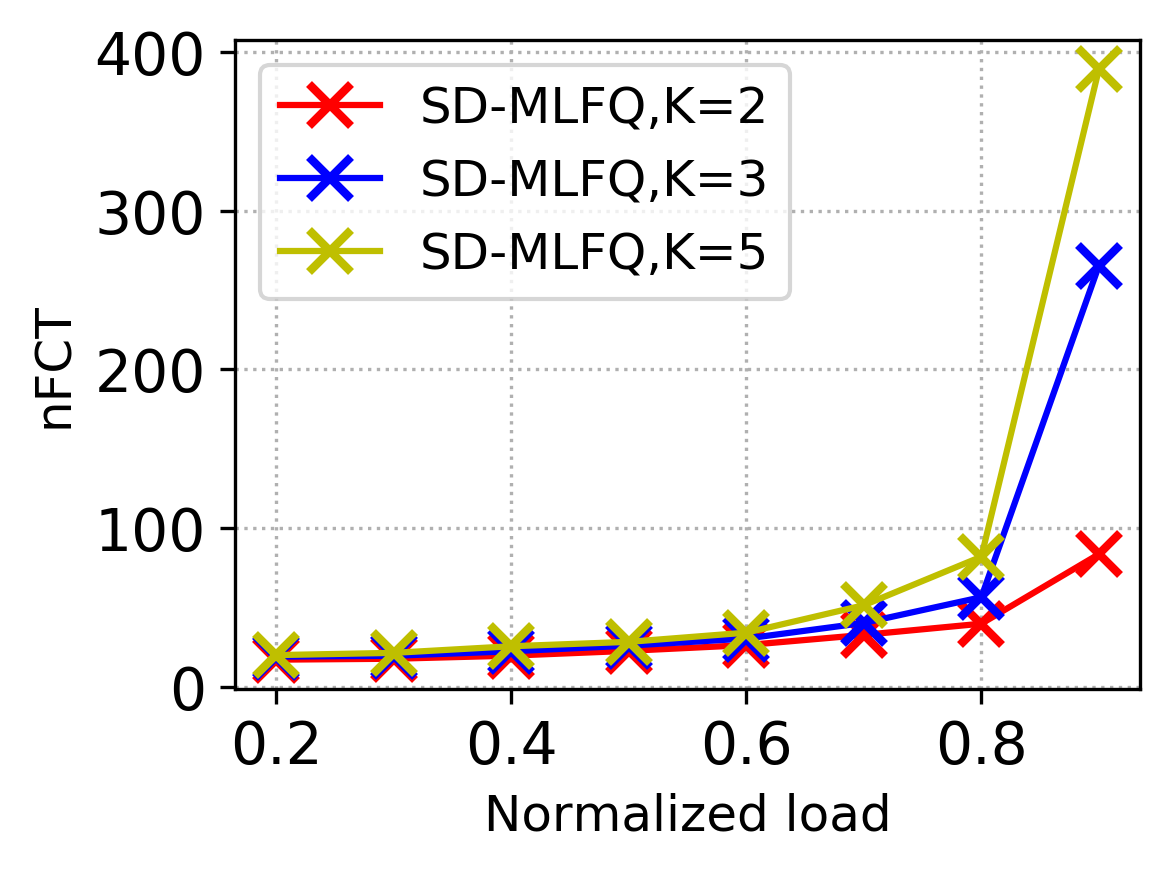
\includegraphics[width=0.4\textwidth]{Chapter4/Figures/sd-larger-topology}
	\caption{SD-MLFQ average nFCT for different $K$}
	\label{fig:sdmlfq_varying_K}
\end{figure}%
Secondly, we compare, for such small topologies, the system employing spatial diversity (SD-MLFQ) with two MLFQ schedulers that use two different threshold sets, optimized and non-optimized. They are PIAS and ES-N, respectively.
\begin{figure}
	\centering
	\begin{subfigure}{.5\textwidth}
		\centering
		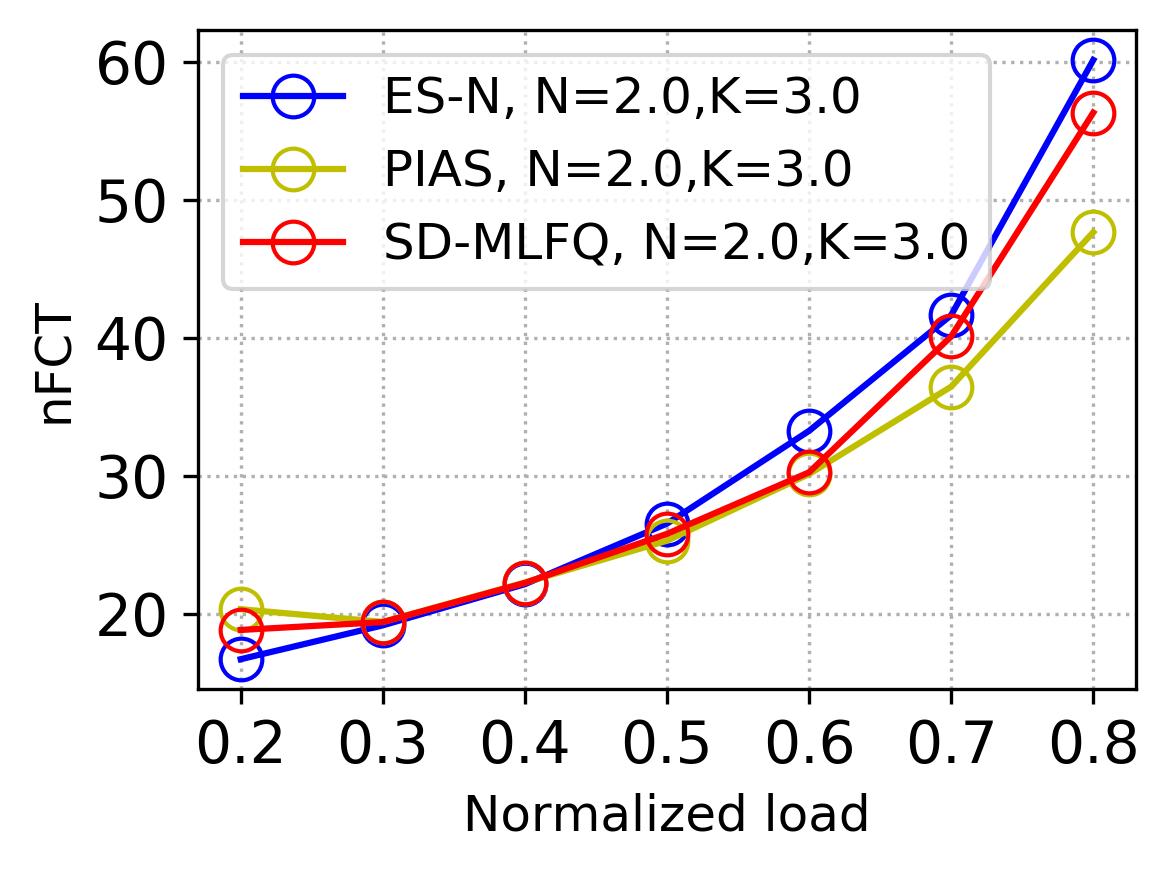
\includegraphics[width=0.8\textwidth]{Chapter4/Figures/sd-final-comparison-fct-vs-load}
		\caption{Average nFCT ($K$=3 only)}
		\label{fig:sd-final}
	\end{subfigure}%
	\hfill
	\begin{subfigure}{.5\textwidth}
		\centering
		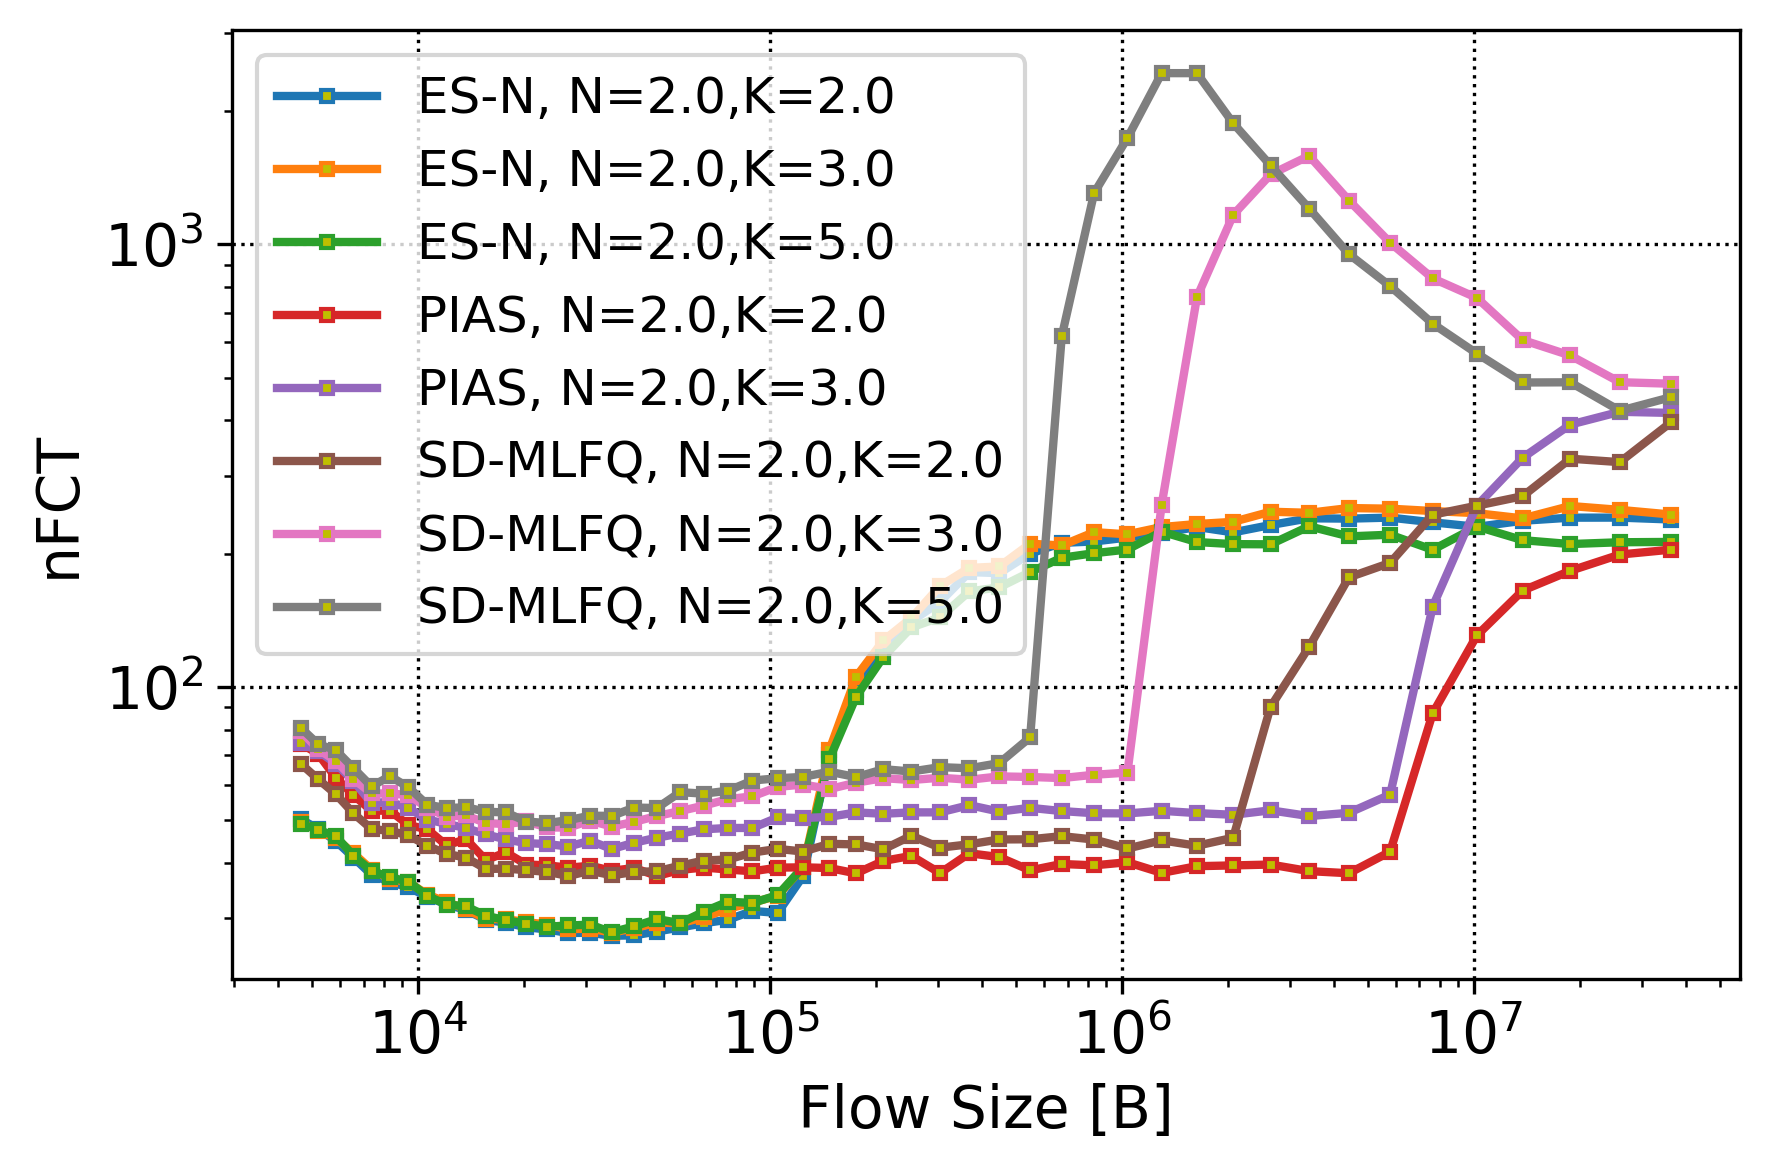
\includegraphics[width=0.99\textwidth]{Chapter4/Figures/sd-final-comparison}
		\caption{nFCT detailed ($\rho$=0.9)}
		\label{fig:sd-final-detailed}
	\end{subfigure}%
	\caption{Final comparison among spatial diversity and other}
	\label{fig:sd-defeat}
\end{figure}%
Unfortunately, from Figure \ref{fig:sd-final} we mainly infer undesired effects with spatial diversity. For all systems, there is a clear FCT variation around the first demotion threshold. We call it $\alpha^{*}$. The ES-N threshold setting  provides best performances on mice flows getting a small $\alpha^{*}$, instead PIAS trades mice response time with medium, by optimizing $\alpha^*$ on the workload distribution, and achieves best average nFCT. Instead, SD-MLFQ gives an unacceptable penalty for flows above $\alpha^*$, even beyond the expectations based on the numerical flow simulator (note that $y$-axis is in log-scale). This essentially tells two things: the additional priority levels offered by spatial diversity do not bring any gain, rather they have a negative effect, while the only influence on the FCT is yielded by the strict priority scheduler around the first threshold. 
%\begin{figure}[!tb]
%	\centering
%	\begin{subfigure}{.5\textwidth}
%		\centering
%		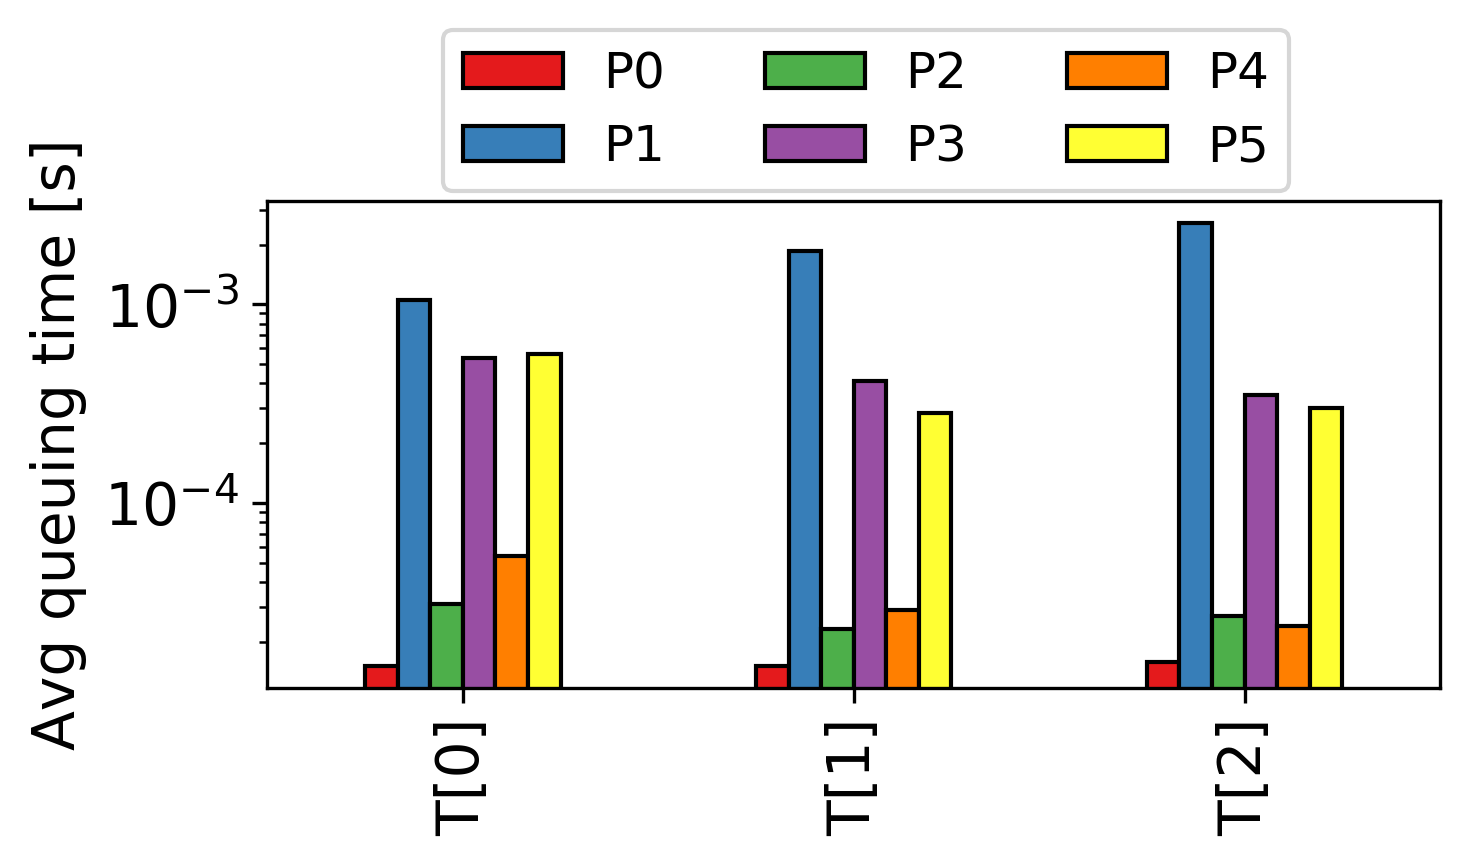
\includegraphics[width=0.99\textwidth]{Chapter4/Figures/sd_priority_queues_tors}
%		\caption{ToR up-send PQ}
%	\label{fig:priority-inversion-tor}
%	\end{subfigure}%
%	\hfill
%	\begin{subfigure}{.5\textwidth}
%		\centering
%		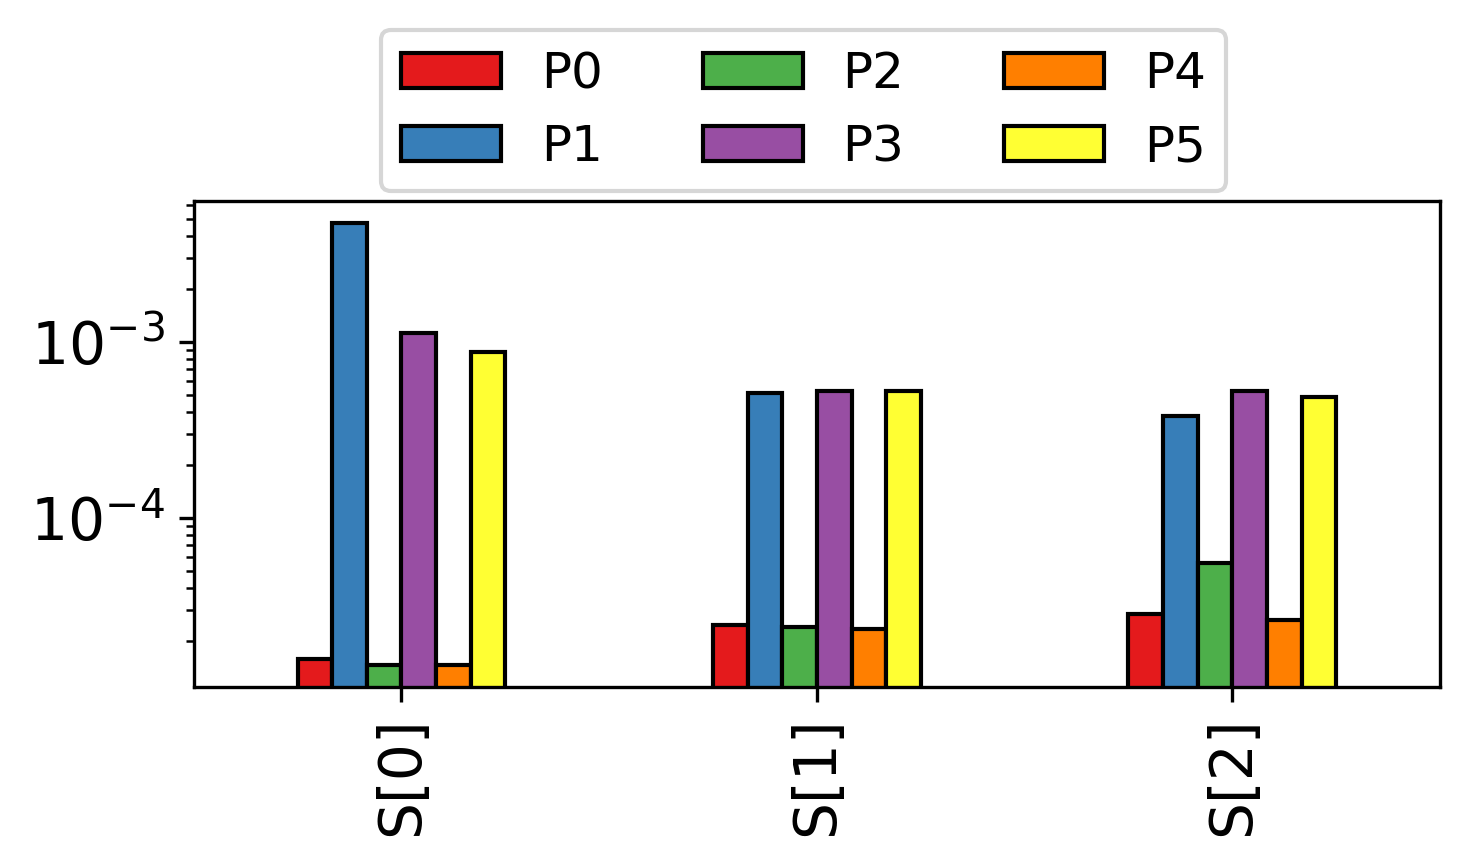
\includegraphics[width=0.99\textwidth]{Chapter4/Figures/sd_priority_queues_spine}
%		\caption{Spine down-send PQ}
%		\label{fig:priority-inversion-spine}
%	\end{subfigure}%
%	\captionsetup{width=0.8\linewidth, justification=centering}
%	\caption{Average packet waiting time in PQ with spatial diversity. $K$=3 and 90\% load.}
%	\label{fig:priority-inversion}
%\end{figure}%
\begin{figure}[!tb]
	\centering
	\begin{subfigure}{.6\linewidth}
		\hspace{6pt}
		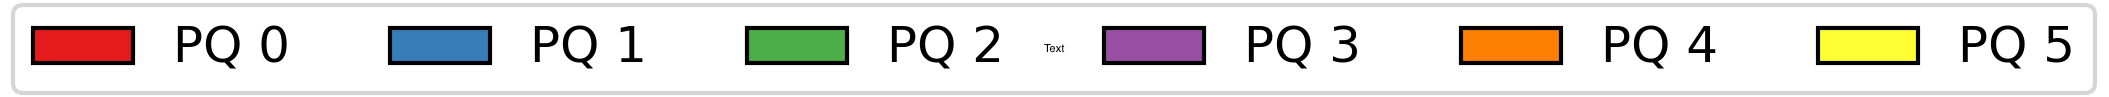
\includegraphics[width=0.99\textwidth]{Chapter4/Figures/legend}
	\end{subfigure}%
	\vfill
	\centering
	\begin{subfigure}{.5\textwidth}
		\centering
		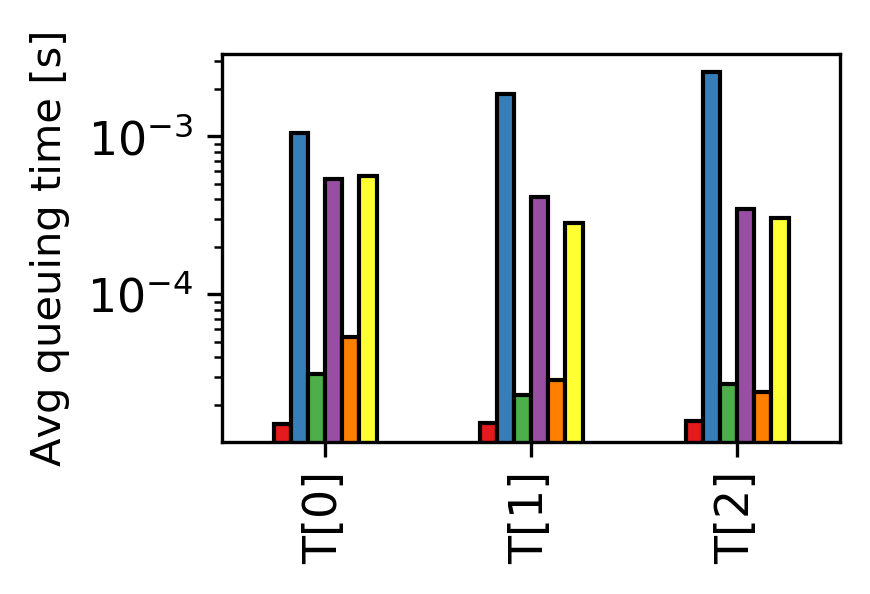
\includegraphics[width=0.7\textwidth]{Chapter4/Figures/sdmlfq-sp-tor_3x2}
	\end{subfigure}%
	\hfill
	\begin{subfigure}{.5\textwidth}
		\centering
		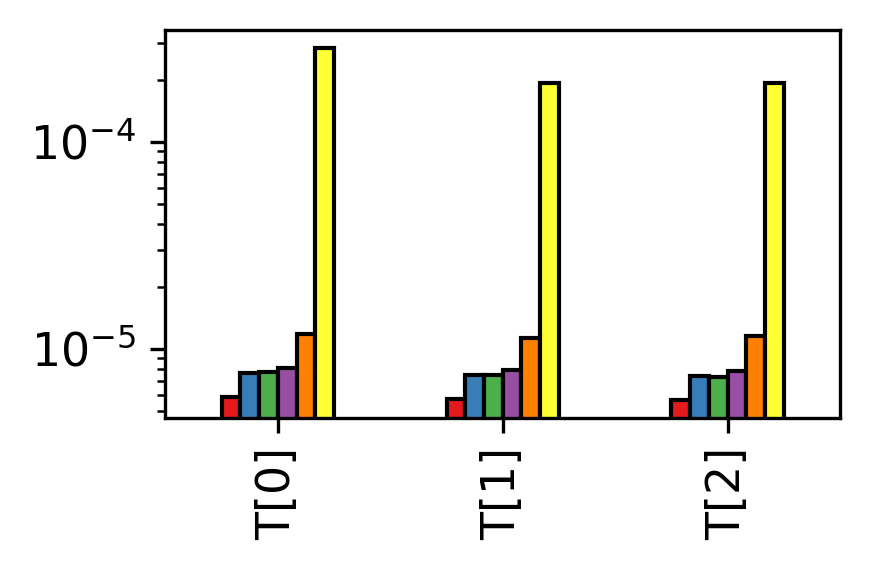
\includegraphics[width=0.7\textwidth]{Chapter4/Figures/esn-sp-tor_3x2}
	\end{subfigure}%
	\vfill
	\begin{subfigure}{.5\textwidth}
		\centering
		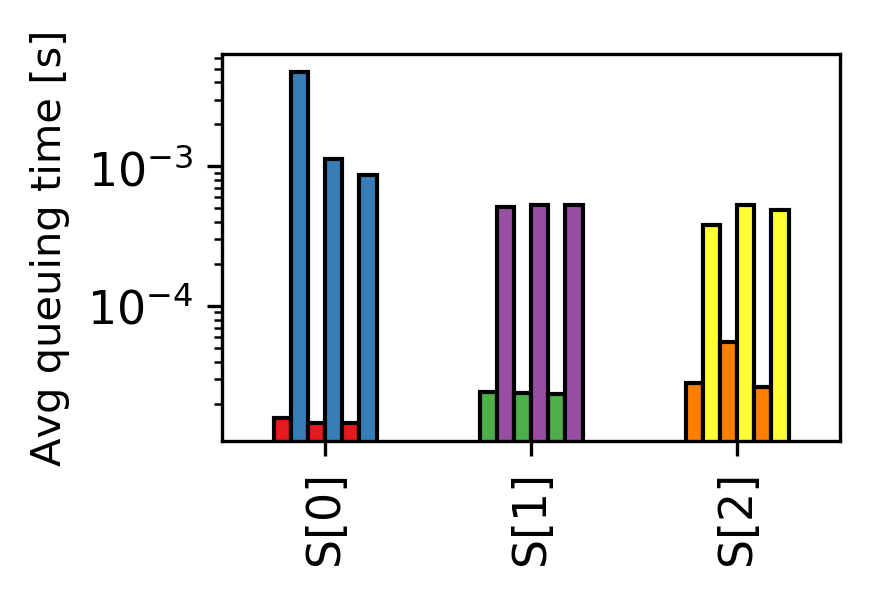
\includegraphics[width=0.7\textwidth]{Chapter4/Figures/sdmlfq-sp-spine_3x2}
		\caption{SD-MLFQ, KN=6}
		\label{fig:strict-priority-inversion-sdmlfq}
	\end{subfigure}%
	\hfill
	\begin{subfigure}{.5\textwidth}
		\centering
		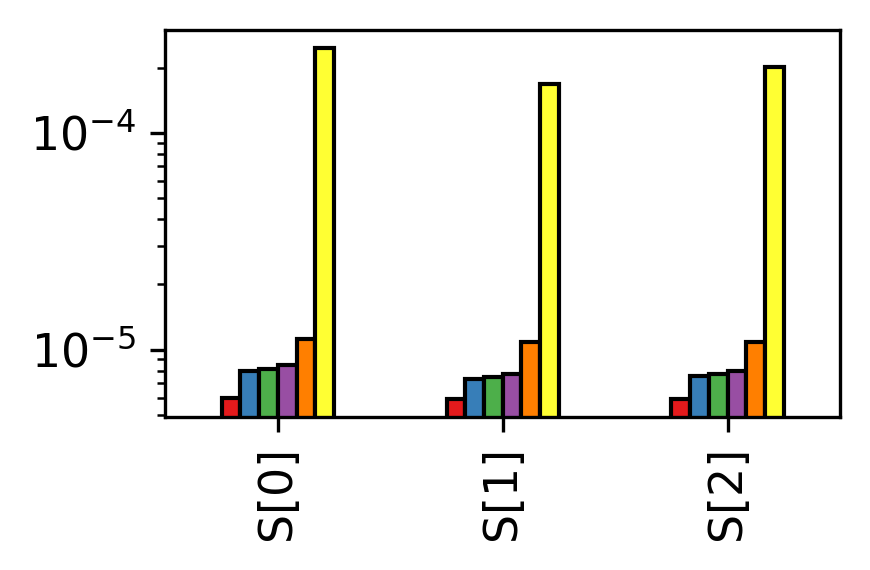
\includegraphics[width=0.7\textwidth]{Chapter4/Figures/esn-sp-spine_3x2}
		\caption{MLFQ, N=6}
		\label{fig:strict-priority-mlfq}
	\end{subfigure}%
%	\captionsetup{width=0.8\linewidth, justification=centering}
	\caption{Average packet waiting time in PQs with and without spatial diversity for K=3 at 90\% load. On $x$-axis ToR \textit{up-send} interfaces and Spine \textit{down-send} interfaces.}
	\label{fig:priority-queuing-time}
\end{figure}%
We wondered why more priorities in SD-MLFQ do not result in any little benefit for medium flows and why there is a sudden FCT deterioration. Indeed, out first intuition was that SD-MLFQ would in principle offer higher granularity to advantage medium flows. Thus, we expected to emulate with only $N$=2 priority queues the performance of a MLFQ system with $N$>2 and to get a trend close to the one of Fig.\ref{fig:esn_varying_N}.

We derived from the simulation in the DCN some additional insights that lead to the following reasoning as a possible explanation. First, we have already seen how the priority-dependent load balancing distributes non uniformly the number of simultaneous flow on the spines, creating some peaks in the queues of high priority spine. Eventually, we noted another aspect. Consider again Fig.\ref{fig:downsend} and the down-send transmission from spines to top-of-rack switches. A key fact is the absence of a scheduler disciplining the transmission among priority queues of different spines. In other words, packets with a priority greater than 1 does not have any dependence from the higher priority packets. Call HP (High-Priority) all queues $Q_0^j(0 \leq j \le K)$ that are given high priority by the SP schedulers, and LP (Low-Priority) all the other queues $Q_1^j(0 \leq j \le K)$. The notation is the same already proposed in Table \ref{tab:queuingmodel}. In the example of Figure \ref{fig:downsend} HP$ = \{0,2,4,6\}$ and LP $ = \{1,3,5,7\}$. %TODO new table
Since there is no coordination among different switches, packets stored in HP have always shorter waiting times than packets in LP, even when they in theory belong to a lower (/higher) priority class (/index). This is illustrated in the histograms of Fig.\ref{fig:strict-priority-inversion-sdmlfq} for 3x3 scenario. Each cluster of bars puts together all priorities available at a given switch. There are $K \times N$ priority queues per switch in total, in this case $3 \times 2 = 6$. Notice how the average queuing time at priority 2 and 4 is shorter than at priority 1. This is not the behavior that would have been obtained with the corresponding MLFQ systems where all $N$ priorities are condensed in the same interface, shown in Fig.\ref{fig:strict-priority-mlfq}. In other words, the actual delays are often in contradiction with the priority class. \\
In general, we think it is very hard to regulate the transmission from SD-MLFQ priority queues physically distributed in different interfaces. First of all, it is very challenging to implement a centralized/distributed signaling mechanism, since queues are not in the same hardware board we cannot convey the scheduling choice with a \emph{speedup} in respect to the link bandwidth. Furthermore, even assuming to manage this limitation, the scheduling problem is complicated. Actually, at a given time instant the down-send spine ports may contain Head-of-Line (HoL) packets destined to different ToRs, or to the same ToR but to different servers. Thus, enforcing as a scheduling criterion the priority alone, would be \emph{non work-conserving} and worse the performance. 
